\documentclass[a4paper]{article}

% --- Page layout and spacing ---
\usepackage[top=3cm, left=3.5cm, right=3.5cm, bottom=3cm]{geometry}
\usepackage[utf8]{inputenc}      % input encoding
\usepackage[T1]{fontenc}         % font encoding
\usepackage[english]{babel}
\usepackage{setspace}
\setlength{\parindent}{0pt}      % paragraph indentation
\setlength{\parskip}{0.8em}      % space between paragraphs
\setstretch{1.2}                 % line spacing
\usepackage{tocloft}             % section spacing in ToC
\usepackage{booktabs}
\setlength{\cftbeforesecskip}{10pt}
\setlength{\cftbeforesubsecskip}{4pt}
\usepackage{titlesec}            % section title spacing
\titlespacing*{\section}{0pt}{5.0ex plus 1ex minus .2ex}{1.0ex plus .2ex}
\titlespacing*{\subsection}{0pt}{3.0ex plus .5ex minus .2ex}{0.8ex plus .2ex}
\titlespacing*{\subsubsection}{0pt}{2.0ex plus .5ex minus .2ex}{0.8ex plus .2ex}

% --- Math and symbols ---
\usepackage{amsmath, amssymb}    % standard math
\usepackage{empheq}              % boxed equations etc.
\DeclareMathOperator{\artanh}{artanh}
\DeclareMathOperator{\sgn}{sgn}
\usepackage{bm}                  % bold math symbols
\usepackage{cancel}              % strikeout in math
\usepackage{siunitx}             % proper units
\DeclareSIUnit\angstrom{\text{Å}}
\renewcommand{\arraystretch}{0.7}

% --- Graphics and floats ---
\usepackage{graphicx}
\usepackage{float}
\usepackage{wrapfig}
\usepackage[justification=centering]{caption}
\usepackage{subcaption}
\captionsetup[figure]{font=small}

% --- Layout helpers ---
\usepackage{boxedminipage}
\usepackage{enumitem}
\usepackage{afterpage}
\usepackage{changepage}
\usepackage{pdfpages}           % include external PDFs
\usepackage{esvect}             % nice vector arrows
\usepackage{hyperref}           % hyperlinks

% --- Bibliography setup ---
\usepackage{csquotes}
\usepackage[backend=biber,style=numeric,sorting=none]{biblatex}
\addbibresource{references.bib}

% --- Fonts ---
\usepackage{lmodern}            % Computer Modern look across TeX distros

\begin{document}

% --- Title page ---
\begin{titlepage}
  \thispagestyle{empty}
  \begin{center}

    % Title
    \vspace*{1cm}
    {\LARGE \textbf{Quadrupole Mass Spectrometer}}\\[1.2cm]

    % Subtitle
    {\large Evaluation Report}\\[2cm]

    % Authors
    \large
    \textbf{Cem Boyaci}\\[-1mm]
    {cemb93@zedat.fu-berlin.de}\\[1cm]

    \textbf{Javier Bellido Roldán}\\[-1mm]
    {bellidoroj98@zedat.fu-berlin.de}\\[1cm]

    \textbf{Leon Goldammer}\\[-1mm]
    {lg4278fu@zedat.fu-berlin.de}\\[6cm]

    % Tutor
    \normalsize
    {Tutor: Kati Hubmann}\\[1.2cm]

    % Footer block
    \textbf{Fortgeschrittenenpraktikum, WS 2025/2026}\\
    Berlin, 28.01.2026\\
    Freie Universität Berlin\\
    Fachbereich Physik

  \end{center}
\end{titlepage}

% --- Table of contents ---
\clearpage
\renewcommand*\contentsname{\huge Contents}
{
  \pagenumbering{gobble}
  \tableofcontents
  \clearpage
}
\pagenumbering{arabic}

% --- Introduction ---
\newpage
\setcounter{page}{1}

\section{Introduction}

Mass spectrometry is a versatile analytical technique used to investigate the composition of atomic and molecular species and plays an important role in many areas of modern science.
In physics and chemistry, it is widely applied whenever gas mixtures or residual gases need to be analyzed with high sensitivity and selectivity.
Among the various types of mass spectrometers, the quadrupole mass spectrometer (QMS) stands out due to its compact design, robustness, and suitability for operation in high vacuum (HV) and ultra-high vacuum (UHV) environments.
For this reason, it has become a standard tool in vacuum diagnostics, residual gas analysis (RGA), and experimental research setups~\cite{jousten_ellefson_partialdruckmessung_2017}.

In this experiment, gas samples are ionized, mass-selected by a quadrupole mass filter (QMF), and detected as an electrical signal, resulting in characteristic mass spectra.
Different gases and gas mixtures are examined, allowing their composition and fragmentation patterns to be analyzed.
In addition, the influence of experimental parameters such as applied voltages, pressure conditions, and operating modes on mass resolution, transmission, and signal quality is investigated.
The measurements provide a practical basis for the interpretation of mass spectra and the assessment of the performance limits of a QMS.

% --- Physical Principles ---
\section{Physical Principles}

In this section, the physical principles underlying the operation of a QMS are outlined.
The discussion follows the path of the particles through the instrument, from ionization and transport under vacuum conditions to mass-selective filtering, detection, and the interpretation of the resulting mass spectra.

\subsection{Mass Spectrometry and Ionization}

Mass spectrometry provides information about the composition of atomic and molecular species by separating ions according to their mass-to-charge ratio.
Since neutral atoms and molecules cannot be manipulated by electric fields, the species under investigation must first be converted into electrically charged ions.
The measured quantity in a mass spectrometer is therefore not the mass itself, but the ratio of mass to charge state $m/z$, where $m$ denotes the ion mass and $z$ the (dimensionless) charge state.
The corresponding physical charge is $Q = ze$, with $e$ the elementary charge.
Different ions with the same mass but different charge states are thus separated at different $m/z$ values, while ions of different mass may appear at similar $m/z$ positions if their charge states differ.
For example, an ion with mass $m$ and $z=1$ and an ion with mass $2m$ and $z=2$ both appear at the same $m/z$ value.

A mass spectrometer generally consists of three essential components: an ion source, a mass-selective analyzer, and an ion detector.
In the ion source, neutral gas particles are ionized and accelerated into the analyzer region.
The analyzer separates the ions according to their $m/z$ value using electric or magnetic fields, and the transmitted ions are finally detected and converted into an electrical signal.
A schematic overview of these basic components is shown in Fig.~\ref{fig:mass_spectrometer}.
In the present experiment, mass selection is performed by a QMF operating with time-dependent electric fields~\cite{QMSAnleitung}.

\begin{figure}[H]
  \centering
  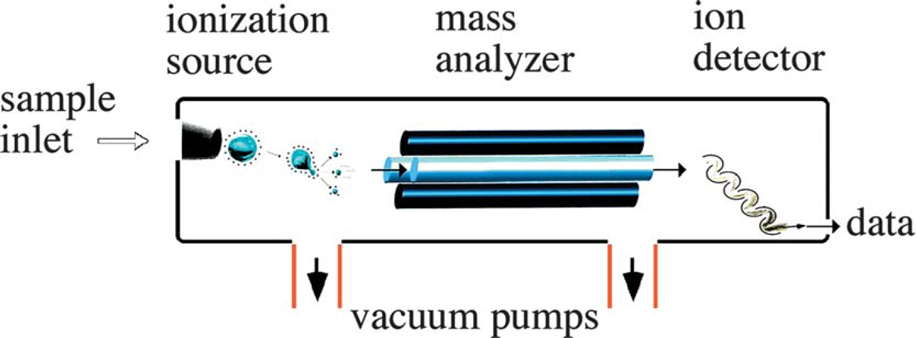
\includegraphics[width=0.95\linewidth]{../resources/figures/mass_spectrometer.png}
  \caption{Schematic overview of the main components of a mass spectrometer, consisting of an ionization source, a mass analyzer, and an ion detector, operated under vacuum conditions~\cite{siuzdak_ms_ionization}.}
  \label{fig:mass_spectrometer}
\end{figure}

Ionization in the QMS used in this experiment is achieved by electron impact ionization.
Electrons are emitted from a heated filament by thermionic emission and accelerated to energies typically on the order of several tens of electronvolts.
When these electrons collide with neutral gas molecules, they can remove an electron and thereby produce positive ions.
Due to the relatively high electron energies, this process often transfers excess energy to the molecule, leading to the formation of fragment ions in addition to the molecular parent ion.

As a consequence, a measured mass spectrum generally consists of multiple peaks corresponding to different ionic fragments of the same molecule.
These fragmentation patterns are characteristic for a given species and can be used to identify unknown gases or gas mixtures.
Under typical operating conditions of electron impact ionization, singly charged ions ($z = 1$) are predominantly observed, so that the measured mass-to-charge ratio $m/z$ closely corresponds to the molecular or fragment mass $m$.
Multiply charged ions may occur but usually do not play a dominant role in RGA~\cite{demtroeder_atome_molekuele_2005}.

\subsection{Vacuum Requirements and Mean Free Path}

The operation of a mass spectrometer requires high vacuum conditions in order to ensure collision-free motion of ions between the ion source, the mass analyzer, and the detector.
At elevated pressures, frequent collisions with background gas molecules would disturb the ion trajectories, lead to energy loss and scattering, and thereby degrade mass resolution and transmission.
Vacuum conditions are therefore an essential prerequisite for reliable mass-selective filtering and accurate interpretation of measured mass spectra.

The relevance of vacuum quality can be quantified by the mean free path $\lambda$ of gas particles, which describes the average distance traveled between successive collisions.
For an ideal gas, the mean free path is given by
\[
  \lambda = \frac{k_{\mathrm{B}} T}{\sqrt{2}\,\pi d^{2} p},
\]
where $k_{\mathrm{B}}$ is the Boltzmann constant, $T$ the temperature, $d$ the effective molecular diameter, and $p$ the gas pressure~\cite{wiki_mean_free_path}.
For fixed $T$ and $d$ this implies $\lambda \propto 1/p$, so lowering the pressure directly increases the collision-free flight distance.
A sufficiently large mean free path compared to the characteristic dimensions of the mass spectrometer is required to ensure that ions can traverse the analyzer region without significant collisional perturbations.

Quadrupole mass spectrometers are therefore typically operated in the HV to UHV regime.
In RGA, pressures on the order of $10^{-6}\,\mathrm{mbar}$ or lower are commonly required, corresponding to mean free paths that far exceed the length of the quadrupole rods~\cite{jousten_ellefson_partialdruckmessung_2017}.

\subsection{Principle of the Quadrupole Mass Filter}

The QMF separates ions according to their mass-to-charge ratio by means of a time-dependent electric quadrupole field.
It consists of four parallel metallic rods arranged symmetrically around the ion beam axis, with opposite rods electrically connected.
Ideally, the electrodes would have hyperbolic cross sections in order to generate a perfect quadrupole field, but in practice cylindrical rods are used as a good approximation~\cite{demtroeder_atome_molekuele_2005}.

A static electric quadrupole potential has a saddle-shaped structure.
This means that ions are focused toward the axis in one transverse direction, while they are simultaneously defocused in the perpendicular direction.
In other words, static quadrupole fields can act like a lens in one plane, but they necessarily act like an anti-lens in the other plane.
Therefore, purely static operation cannot provide stable confinement in both transverse directions at the same time, and ions are inevitably driven into the rods.
Stable transmission through the quadrupole is therefore only achieved by superimposing a static (DC) voltage with an alternating radio-frequency (RF) voltage applied to the rod pairs with opposite polarity.

The superposition of DC and RF voltages produces a time-dependent electric field in which ions perform oscillatory motion perpendicular to the flight direction.
Depending on their mass-to-charge ratio, these oscillations can either remain bounded or grow in amplitude until the ion collides with one of the rods.
Only ions whose trajectories remain stable in both transverse directions are able to pass through the quadrupole and reach the detector, while all others are filtered out.
This principle is illustrated schematically in Fig.~\ref{fig:qmf_principle}.

\vspace{1em}
\begin{figure}[H]
  \centering
  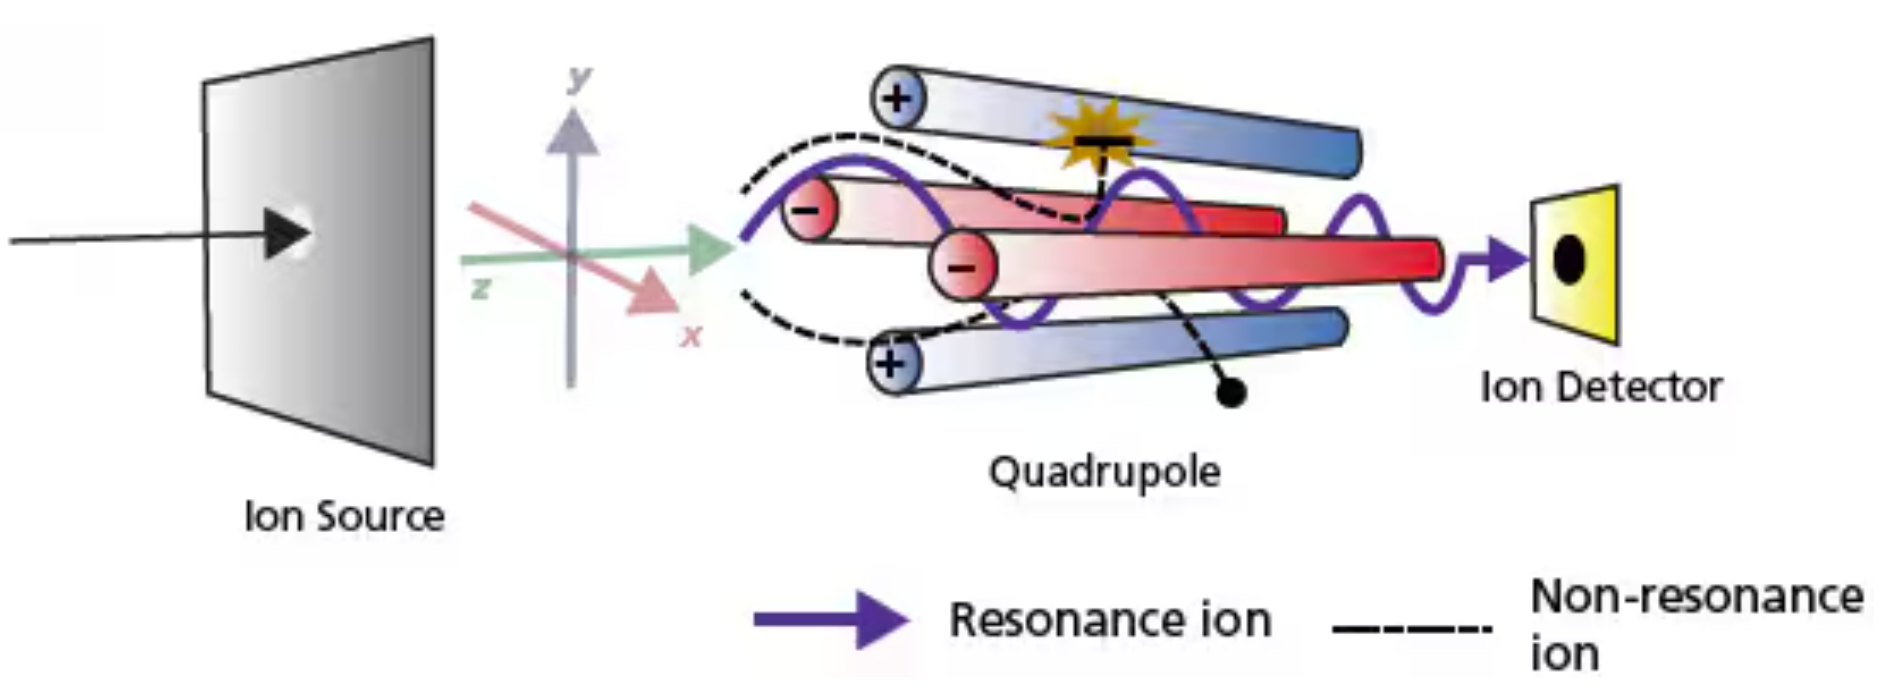
\includegraphics[width=0.95\linewidth]{../resources/figures/qmf_principle.png}
  \caption{Schematic illustration of ion motion in a QMF.
  Ions with suitable mass-to-charge ratios exhibit stable oscillatory trajectories and are transmitted to the detector, while ions with unstable motion are lost to the electrodes~\cite{shimadzu_mass_analyzers}.}
  \label{fig:qmf_principle}
\end{figure}

By varying the applied DC and RF voltages while keeping their ratio constant, the QMF can be operated as a mass-selective device.
In this mode, ions are transmitted sequentially according to their mass-to-charge ratio, allowing a mass spectrum to be recorded.
The detailed conditions for stable and unstable ion motion are described by the equations of motion in the quadrupole field and are discussed in the following subsection.

\subsection{Ion Motion in the Quadrupole Field}

After their creation in the ion source, ions are extracted by an electric field and accelerated toward the quadrupole, which turns their initially random thermal motion into a directed beam along the rod axis.
The corresponding acceleration voltage sets the kinetic energy of the ions and therefore largely determines their forward velocity through the instrument.

Inside an ideal quadrupole field, the electric forces act mainly perpendicular to the flight direction, so the ions are continuously steered sideways while their forward motion along the axis remains approximately uniform.
In the HV regime considered here, collisions are rare on the flight path, so the ions essentially coast through the rod system with a nearly constant axial speed that is set by the extraction energy.

To describe the transverse dynamics, we choose the coordinate system such that the rods are aligned with the $z$-axis and the transverse coordinates are $(x,y)$.
The electric potential in the interior of an ideal quadrupole can then be written as
\[
  \Phi(x,y,t)=\frac{U+V\cos(\omega t)}{2r_0^2}\left(x^2-y^2\right),
\]
where $U$ is the applied DC voltage, $V$ the RF amplitude, and $\omega$ the angular frequency of the RF field~\cite{demtroeder_atome_molekuele_2005}.
The parameter $r_0$ denotes the characteristic field radius, i.e.\ the distance from the axis to the electrode surface in the ideal hyperbolic geometry, so that opposite electrodes are separated by $2r_0$.
This geometrical definition of $r_0$, as well as the electrode arrangement that generates the quadrupole field, is illustrated in Fig.~\ref{fig:qmf_hyperbolic_geometry}.

\vspace{1em}
\begin{figure}[H]
  \centering
  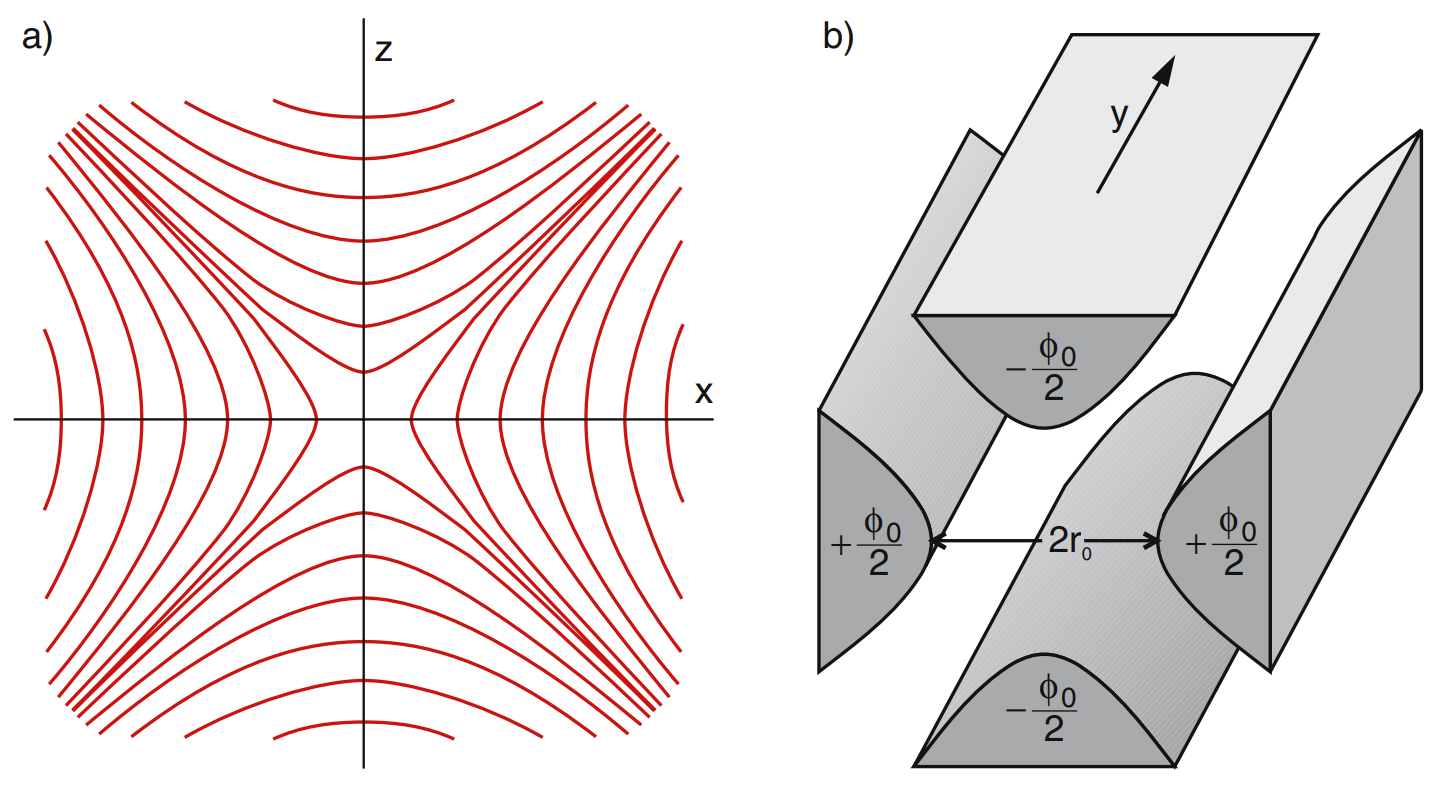
\includegraphics[width=0.95\linewidth]{../resources/figures/qmf_hyperbolic_geometry.png}
  \caption{Ideal quadrupole field generated by hyperbolic electrodes.
    (a) Equipotential lines in the transverse $(x,y)$ plane.
    (b) Schematic cross section of the four hyperbolic electrodes, showing the characteristic field radius $r_0$ and the electrode spacing $2r_0$.
  Adapted from~\cite{demtroeder_atome_molekuele_2005}.}
  \label{fig:qmf_hyperbolic_geometry}
\end{figure}

The saddle-shaped quadrupole potential explains why focusing and defocusing occur simultaneously in perpendicular directions.
A visualization of the saddle potential and its equipotential structure in the transverse plane is shown in Fig.~\ref{fig:qmf_saddle_potential}.

\vspace{1em}
\begin{figure}[H]
  \centering
  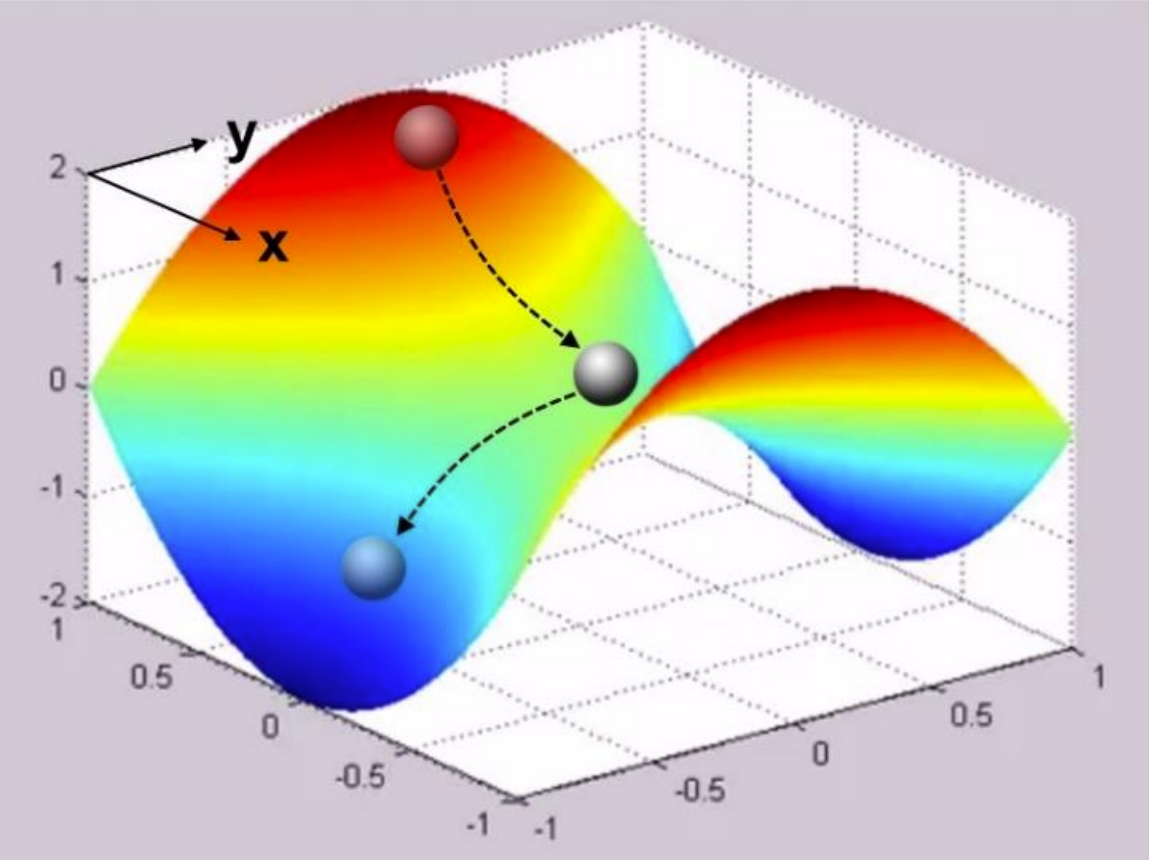
\includegraphics[width=0.9\linewidth]{../resources/figures/qmf_saddle_potential.png}
  \caption{Example visualization of the saddle-shaped quadrupole potential and its equipotential structure in the transverse plane.
  The curvature has opposite sign in $x$- and $y$-direction, which is the origin of the alternating focusing and defocusing behavior~\cite{rwth_mass_spectrometry_2024}.}
  \label{fig:qmf_saddle_potential}
\end{figure}

The ion motion follows from Newton's equation with the electric force $\bm{F}=Q\bm{E}=-Q\nabla\Phi$, where $Q=z_{\mathrm{ch}}e$ is the ion charge and $z_{\mathrm{ch}}$ is the charge state (this $z_{\mathrm{ch}}$ is the same quantity that appears in $m/z$, not to be confused with the spatial coordinate $z$).
Since $\Phi$ is independent of the axial coordinate $z$, the quadrupole field does not provide a direct accelerating or decelerating force along the flight direction, but it strongly affects the transverse motion.
Inserting the potential yields two decoupled equations for $x(t)$ and $y(t)$,
\begin{equation}
  \ddot{x}+\frac{Q}{m r_0^2}\left(U+V\cos(\omega t)\right)x=0,
  \qquad
  \ddot{y}-\frac{Q}{m r_0^2}\left(U+V\cos(\omega t)\right)y=0.
  \label{eq:qmf_eom_xy}
\end{equation}

The opposite signs are the mathematical expression of focusing and defocusing.
A restoring force has the form $\ddot{x}=-\Omega^2 x$ and produces bounded oscillations, as in a harmonic oscillator.
A defocusing force corresponds to $\ddot{y}=+\Omega^2 y$ and leads to runaway solutions whose amplitude grows rapidly, similar to an inverted oscillator.
Therefore, a purely static quadrupole field ($V=0$) can never confine ions in both transverse directions at the same time, because one coordinate is always unstable.

The role of the RF voltage is that it repeatedly alternates the focusing and defocusing action in time.
For certain combinations of $U$, $V$, and $\omega$, this rapid alternation leads to a net dynamic stabilization, so that the transverse oscillations remain bounded in both directions and the ion can pass through the rod system without touching an electrode.
For other parameter combinations, the RF field pumps energy into the transverse motion (a form of parametric instability), and the oscillation amplitude grows until the ion is lost to a rod.
An intuitive, non-mathematical explanation of this is given in~\cite{nizkorodov_qms_youtube_2009}.

Introducing the dimensionless time $\tau=\omega t/2$, Eq.~\eqref{eq:qmf_eom_xy} can be written in the standard Mathieu form,
\begin{equation}
  \frac{d^2 x}{d\tau^2}+\left(a-2q\cos(2\tau)\right)x=0,
  \qquad
  \frac{d^2 y}{d\tau^2}+\left(-a+2q\cos(2\tau)\right)y=0,
  \label{eq:mathieu_xy}
\end{equation}

with the dimensionless parameters
\begin{equation}
  a=\frac{4QU}{m r_0^2\omega^2},
  \qquad
  q=\frac{2QV}{m r_0^2\omega^2}.
  \label{eq:mathieu_aq}
\end{equation}

The parameters $(a,q)$ summarize how strongly the electric field acts on a given ion species.
For fixed instrument settings $(U,V,\omega,r_0)$, they scale with the ratio $Q/m$, so that different $m/z$ values correspond to different points in the $(a,q)$ plane.
Only in certain regions of this parameter plane do the Mathieu solutions stay bounded in both transverse directions, which physically means that the ion oscillations remain finite and transmission through the quadrupole is possible.

\subsection{Stability Diagram and Mass Selection}\label{sec:working_line}

The Mathieu equations in Eq.~\eqref{eq:mathieu_xy} admit either stable or unstable solutions depending on the parameters $(a,q)$.
A trajectory is called stable if the transverse oscillations remain bounded, meaning that the ion stays within the free aperture between the rods over the full flight time.
If the solution is unstable, the oscillation amplitude grows and the ion eventually collides with an electrode and is removed from the transmitted ion beam.

The stability properties are commonly summarized in a stability diagram in the $(a,q)$ plane, where the regions of bounded solutions are indicated.
Only ions whose parameters lie inside a stability region in both transverse directions are transmitted through the quadrupole.
This concept is illustrated in Fig.~\ref{fig:qmf_stability_demtroeder}.

\vspace{1em}
\begin{figure}[H]
  \centering
  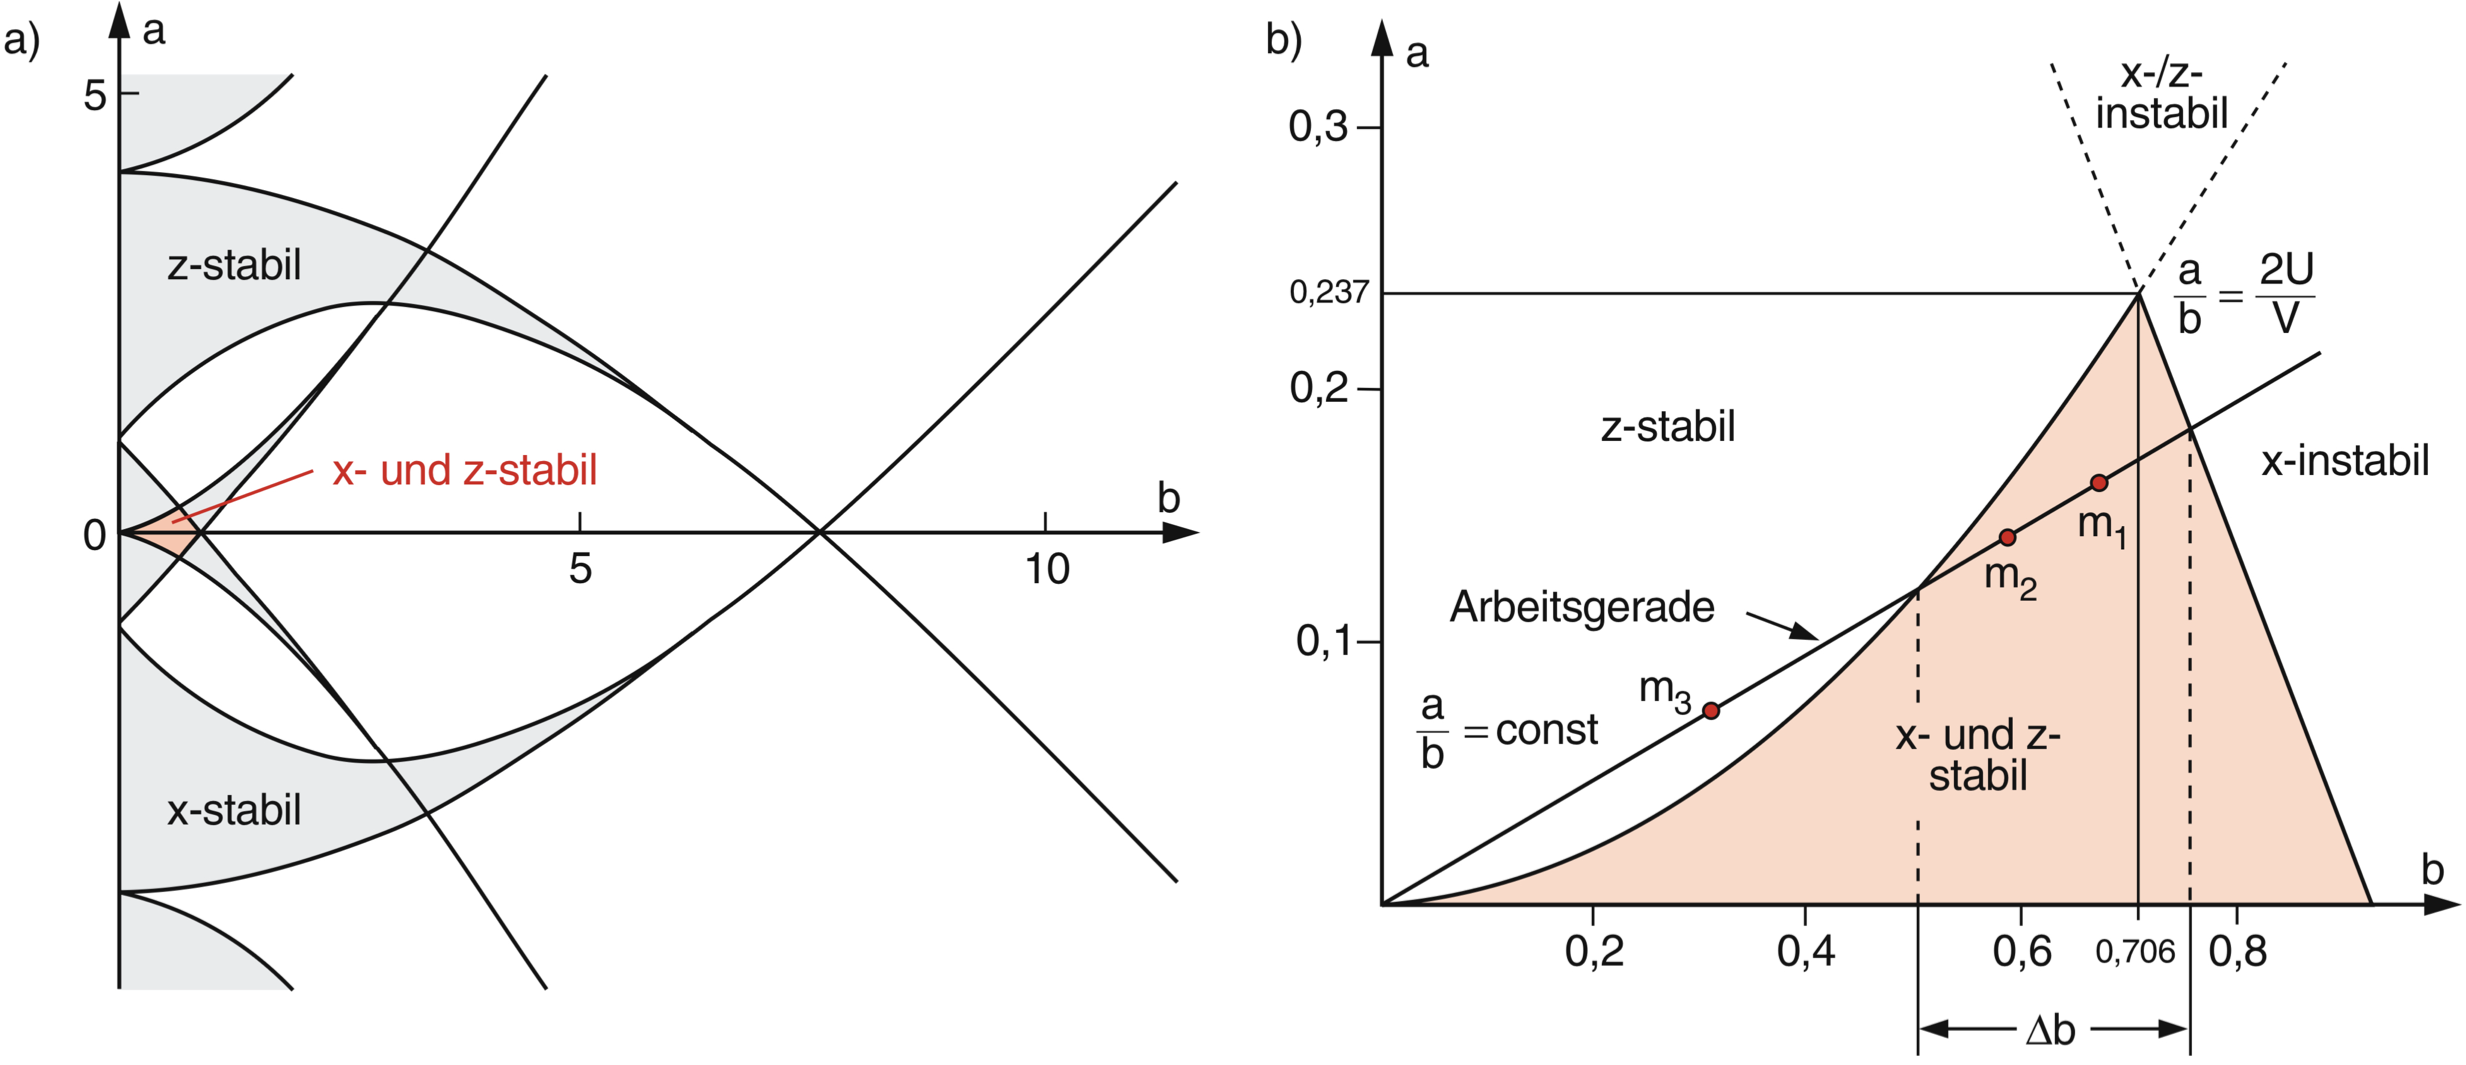
\includegraphics[width=1.0\linewidth]{../resources/figures/qmf_mathieu.png}
  \caption{Mathieu stability diagram and working line principle for a QMF.
    (a) Overview of stability regions in the $(a,b)$ plane, where stability is obtained only if the motion remains bounded in both transverse directions.
    (b) Enlarged view of the first stability region, which is used for mass filtering, together with a straight working line through the origin.
    In the notation of the source, the horizontal axis is labeled $b$ (corresponding to $q$ in this report), and the second transverse coordinate is labeled $z$ (corresponding to $y$ in this report).
  Adapted from~\cite{demtroeder_atome_molekuele_2005}.}
  \label{fig:qmf_stability_demtroeder}
\end{figure}

Mass selection is achieved by operating the quadrupole at parameter values close to the boundary of the first stability region.
Using Eq.~\eqref{eq:mathieu_aq}, the stability parameters scale as $a\propto QU/m$ and $q\propto QV/m$ for fixed $(r_0,\omega)$.
For a fixed ion species, changing $U$ and $V$ moves the operating point in the stability diagram.
In particular, keeping the ratio of DC to RF amplitude constant implies
\[
  \frac{a}{q}=\frac{2U}{V}=\text{const.},
\]
so that the operating point follows a straight line through the origin.
This line is commonly referred to as the working line, and it is shown in Fig.~\ref{fig:qmf_stability_demtroeder}b.

A mass spectrum is recorded by scanning $U$ and $V$ simultaneously while maintaining a constant ratio $U/V$.
Only ions whose $(a,q)$ values lie inside the chosen stability region at a given moment are transmitted to the detector, while ions outside the region are rejected by unstable motion.
Since both $a$ and $q$ are proportional to $Q/m$, heavier ions require higher voltages to reach the same stability conditions.
Therefore, scanning the voltages corresponds to scanning the transmitted mass-to-charge ratio $m/z$.

The position of the working line relative to the stability boundaries determines the trade-off between resolution and transmission.
Choosing a working line closer to the tip of the stability region narrows the transmitted $m/z$ window and increases resolution, but reduces the fraction of ions that remain stable over the full rod length, leading to lower transmission and weaker signal.
This is illustrated in Fig.~\ref{fig:qmf_resolution}, where scanning along the working line selects different ion masses, while the transmitted mass interval $\Delta m$ depends on the line slope.

\vspace{1em}
\begin{figure}[H]
  \centering
  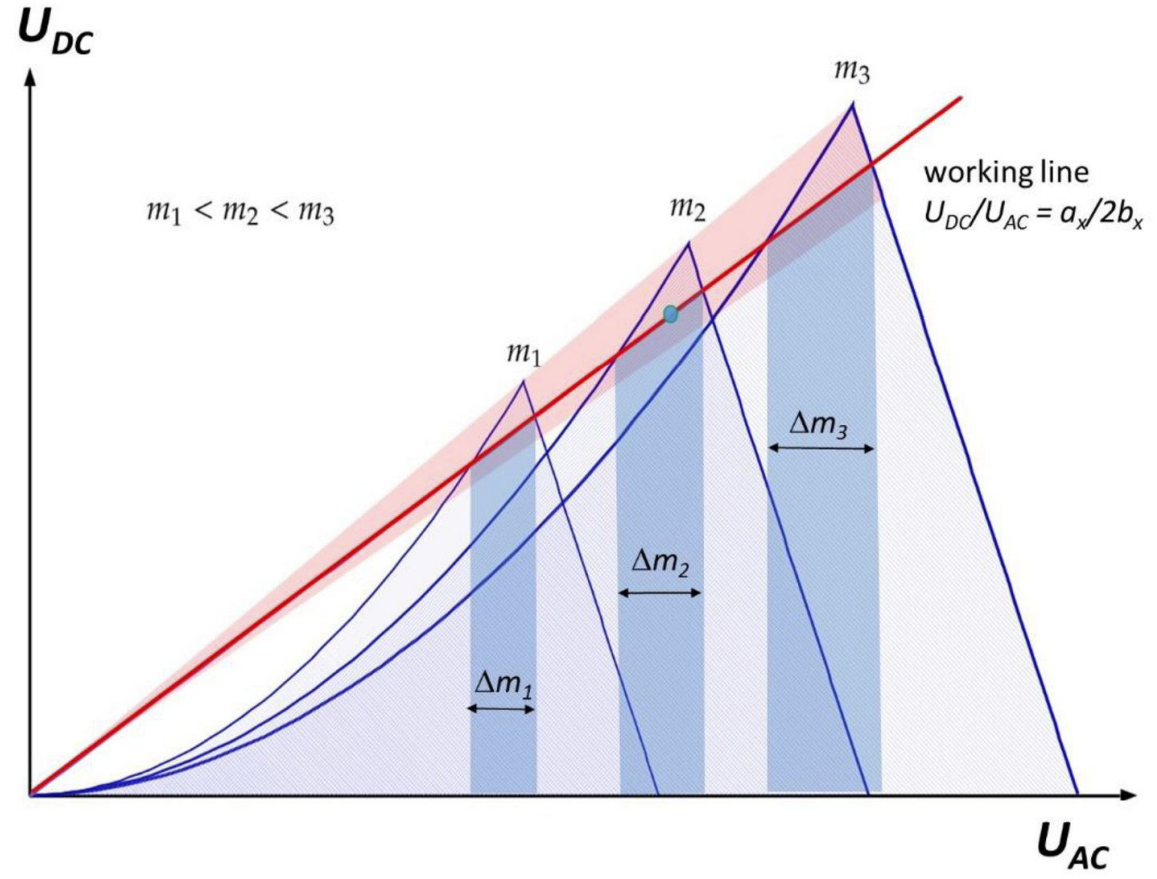
\includegraphics[width=0.85\linewidth]{../resources/figures/qmf_resolution.png}
  \caption{Working line principle and resolution in a QMF.
    Scanning $U$ and $V$ along a straight working line transmits different ion masses $m_1<m_2<m_3$, while the transmitted interval $\Delta m$ depends on the slope.
  In the notation of the source, the voltages are labeled $U_{DC}$ and $U_{AC}$ (corresponding to $U$ and $V$ in this report), and the working line condition is written as $U_{DC}/U_{AC} = a_x/2b_x$ (corresponding to $a/q = 2U/V$ in this report)~\cite{rwth_mass_spectrometry_2024}.}
  \label{fig:qmf_resolution}
\end{figure}

\subsection{Detection and Mass Spectra}
\label{sec:massspectra}

After the quadrupole has filtered the ion beam, the remaining ions are collected by a detector and converted into an electrical signal.
What we ultimately record is a ``mass spectrum'', i.e.\ the detector signal as a function of the selected mass-to-charge ratio $m/z$.
Ideally, the spectrum would show clean, well-separated peaks that can be assigned to gas species.
In practice, however, many peaks are small, some overlap, and the signal often sits on a nonzero background, so detector choice and scan settings determine how reliably weak peaks can still be distinguished from noise.

In the QMS, the detector signal is an ion current.
It can either be measured directly with a Faraday cup or first amplified with an electron multiplier and then measured as an electron current.
A Faraday cup is conceptually simple and very linear, but for very small ion currents the measurement becomes noise-limited.
An electron multiplier increases the current by a large factor (gain), which makes weak peaks much easier to see, but the gain can drift and the amplification adds noise and saturation effects.
In other words, the Faraday cup is preferable when signals are large and linearity is important, whereas the multiplier is useful when the goal is to detect very small signals at all.

Even before interpreting which gases are present, it helps to remember that the QMF does not transmit an infinitely sharp mass value, but always a finite mass window around it.
In an idealized picture this window would be perfectly rectangular, yet real instruments produce broadened and often slightly asymmetric peaks.
Two important reasons are the finite electrode spacing (so transmission depends on the ion’s initial position and angle) and the finite rod length (so some ``almost unstable'' ions still make it through before hitting a rod).
This difference between an ideal and a realistic peak shape is sketched in Fig.~\ref{fig:qmf_peakshape}.

\vspace{1em}
\begin{figure}[H]
  \centering
  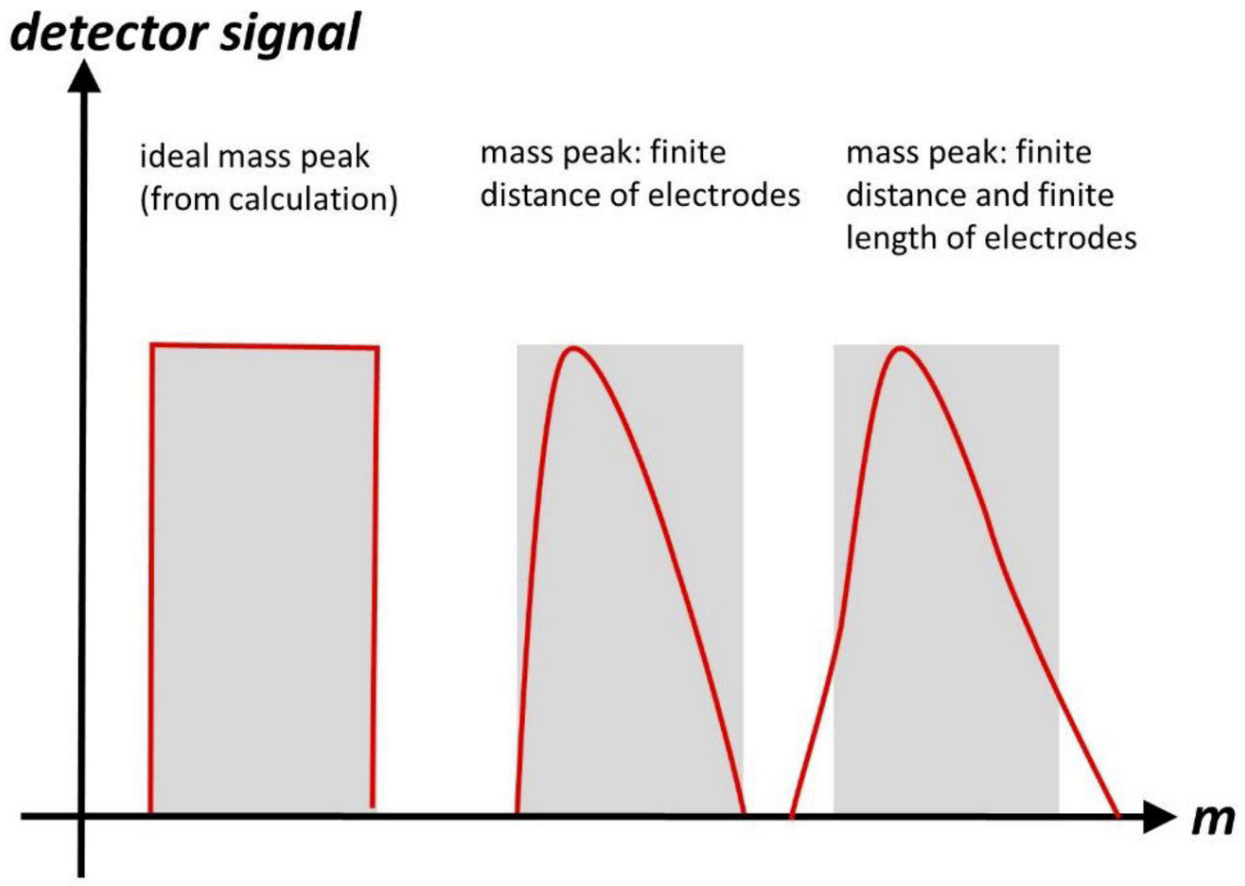
\includegraphics[width=0.86\linewidth]{../resources/figures/qmf_peakshape.png}
  \caption{Idealized versus realistic peak shapes in a QMF.
  Finite electrode spacing and finite rod length broaden the transmission window, turning an ideal rectangular peak into a rounded peak with finite width $\Delta m$~\cite{rwth_mass_spectrometry_2024}.}
  \label{fig:qmf_peakshape}
\end{figure}

A common practical definition of mass resolution is $R=m/\Delta m$, where $\Delta m$ is the full width at half maximum (FWHM) of a peak~\cite{jousten_ellefson_partialdruckmessung_2017}.
Higher resolution (smaller $\Delta m$) usually means lower transmission, because fewer ions remain stable over the full rod length.
So there is a trade-off: higher resolution separates neighboring masses better but reduces signal, whereas higher transmission gives stronger scans but increases overlap and peak tails.
In addition, scan speed (dwell time per mass channel) affects noise: faster scans make weak peaks harder to see, while slower scans improve signal-to-noise but take longer.

Peak positions indicate which ions were transmitted, while peak heights (or areas) reflect how many ions reached the detector.
In RGA, intensity is often used as a proxy for the \emph{partial pressure} of a gas component, but only after accounting for background and sensitivity.
A common step is therefore to record a background spectrum (``rest gas spectrum'') and subtract it, especially when small peaks sit on the shoulders of larger ones.

Peak intensities cannot be read as partial pressures directly, because the measured signal depends on more than just how much of a gas is present.
It also depends on ionization, fragmentation, and transmission probabilities, as well as the chosen measurement settings.
These effects are often bundled into a sensitivity factor $K_i$, so that for a chosen mass channel $i$ one relates partial pressure $p_i$ to ion current $I_i$ via $p_i = I_i/K_i$~\cite{jousten_ellefson_partialdruckmessung_2017}.
If $K_i$ is not known, the spectrum can only be interpreted relatively, and partial pressures obtained from (normalized) peak intensities are only approximate, instrument-dependent estimates.

For identifying gases, the key point is that electron impact ionization produces fragment ions in addition to the molecular parent ion.
A single gas therefore appears as a characteristic pattern of multiple peaks, so identification is typically pattern-based rather than based on one line.
In vacuum systems, water-related peaks around $m/z\approx 18$ and air-related peaks around $m/z\approx 28,32,40$ are common starting points, but assignments become reliable only once the accompanying peaks match the expected fingerprint.

Figure~\ref{fig:acetone_spectrum} illustrates this with a reference spectrum of acetone.
Instead of a single ``acetone line'', the molecular ion appears together with several prominent fragments, and the overall combination makes the identification robust.

\vspace{1em}
\begin{figure}[H]
  \centering
  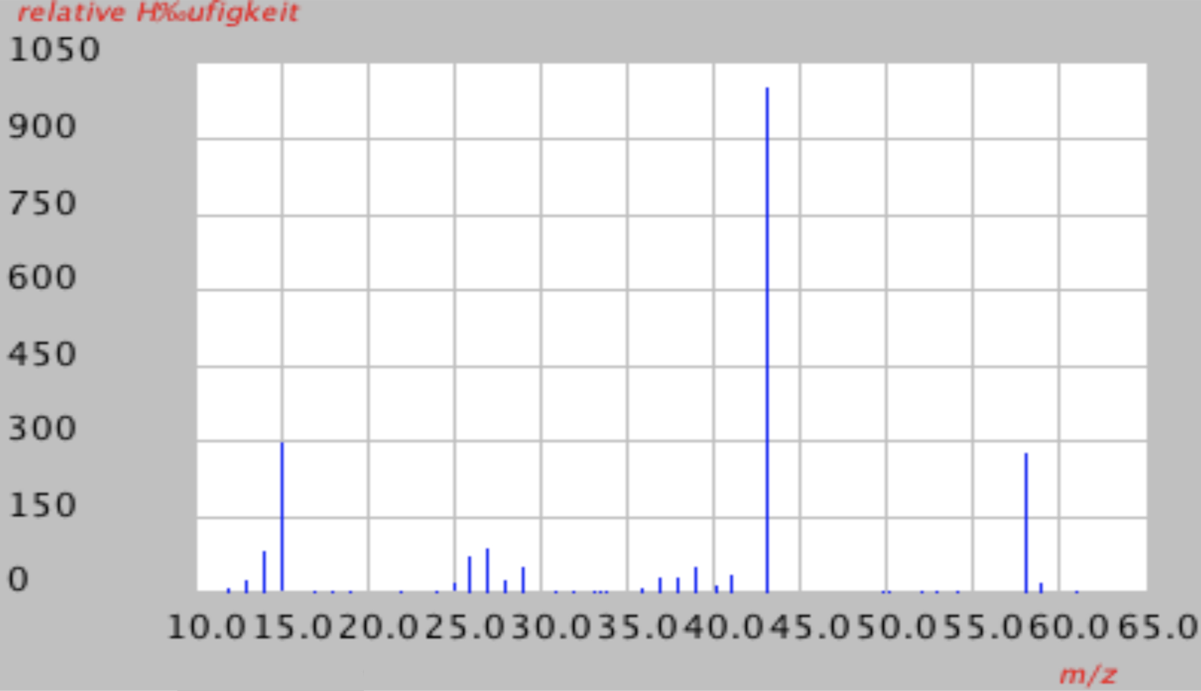
\includegraphics[width=0.83\linewidth]{../resources/figures/acetone_spectrum.png}
  \caption{Example electron-impact mass spectrum of acetone illustrating parent and fragment peaks, as used for pattern-based identification in RGA~\cite{QMSAnleitung}.}
  \label{fig:acetone_spectrum}
\end{figure}

% --- Experimental Setup ---
\section{Experimental Setup}

This section describes the vacuum system, gas handling, and the QMS used for all measurements in this experiment.
The setup is summarized schematically in Fig.~\ref{fig:setup_overview}.

\subsection{Vacuum System and Gas Handling}

All measurements are performed in a stainless-steel vacuum chamber (recipient) that is continuously evacuated during operation.
High-vacuum pumping is provided by a turbomolecular pump mounted directly on the recipient and backed by a mechanical fore-vacuum (membrane) pump.
The turbo pump transfers momentum from rapidly rotating rotor blades to gas molecules and drives them toward the foreline, while the membrane pump removes this gas by periodic volume changes of a diaphragm chamber.

Test gases are supplied from three reservoirs (acetone, ethanol, argon) and from ambient air via a dosing manifold.
Each source can be isolated individually and feeds into a common manifold section.
For flushing between gases, this manifold can be evacuated with a separate rotary vane pump to remove residual gas in the lines.
Admission to the recipient is then controlled by an isolation valve followed by a fine dosing (needle) valve at the chamber inlet.
During dosing, the needle valve is opened gradually while pumping continues, so the pressure rises to a steady value where gas inflow and pumping balance.
A pressure gauge on the manifold monitors the line pressure during flushing and dosing.

\vspace{1em}
\begin{figure}[H]
  \centering
  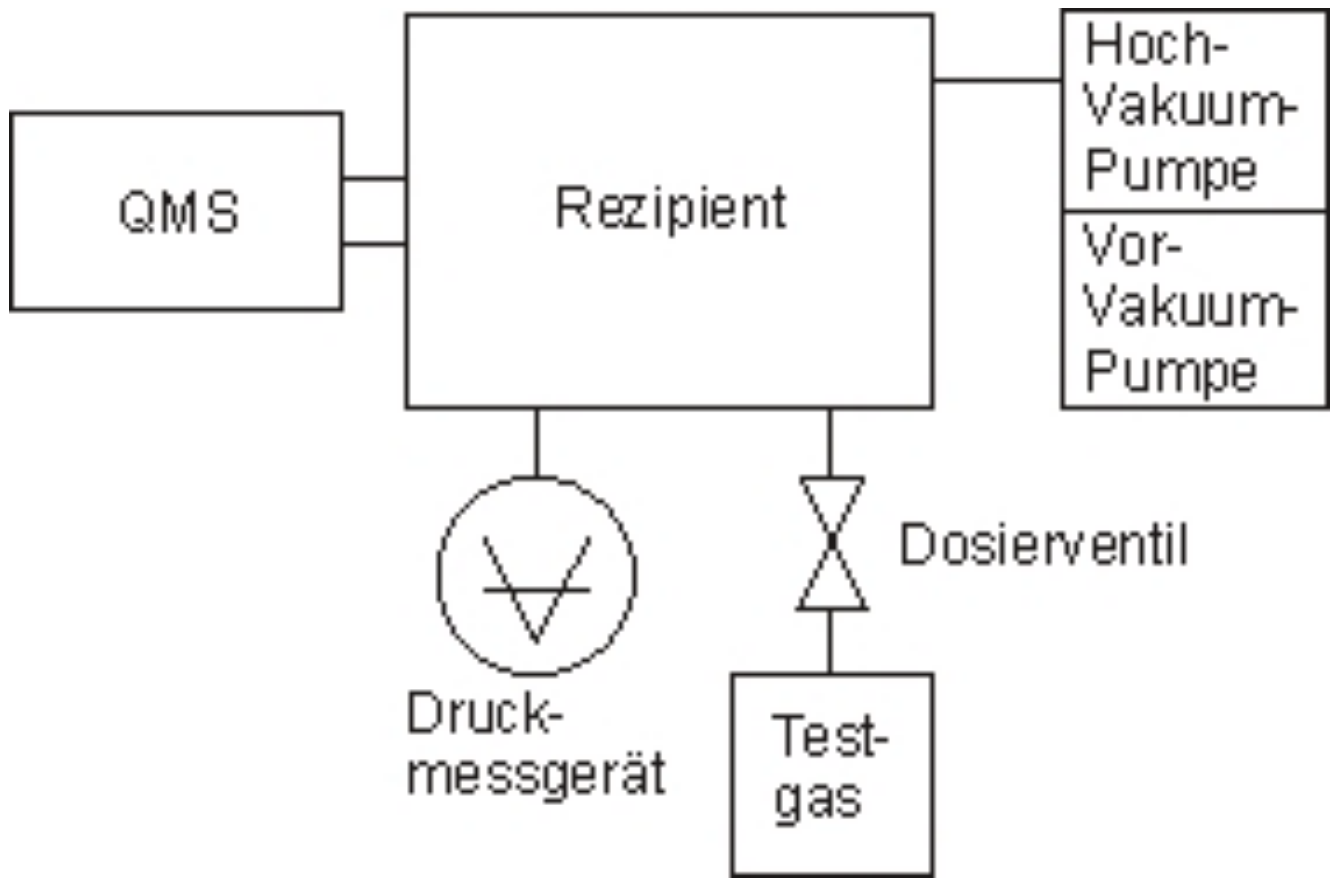
\includegraphics[width=0.8\linewidth]{../resources/figures/schematic_setup.png}
  \caption{Schematic overview of the experimental vacuum setup consisting of the QMS connected to the recipient, the pumping system, the pressure gauge, and the dosing line for test gases~\cite{QMSAnleitung}.}
  \label{fig:setup_overview}
\end{figure}

The total pressure in the recipient is monitored with a cold-cathode ionization gauge mounted directly on the chamber.
A high voltage sustains a gas discharge that ionizes residual molecules, and the resulting discharge current increases with gas density and thus serves as a pressure-dependent signal~\cite{leybold_indirekte_vakuumdruckmesser}.
The gauge reading is used as the reference for setting and reproducing the operating pressure during dosing and evacuation.

\subsection{Quadrupole Mass Spectrometer and Control Electronics}

The QMS measuring head is connected to the recipient via a flange and contains the ion source, the quadrupole rods, and the ion detector inside the vacuum.
All operating voltages are supplied and synchronized by the QMS control unit, which performs the mass scan (output: mass channel) and provides the measured detector signal (output: intensity).

Figure~\ref{fig:setup_electronics} summarizes the connected devices and signal paths.
Two external DC power supplies (100\,V and 200\,V) feed a voltage divider, which provides the required DC voltages for the control unit and for the QMS head.
For mass filtering, the control unit applies a DC component to the quadrupole rods, while an external HF generator supplies the RF (AC) component.
Together they form the time-dependent quadrupole field at the rods.
The ion current at the detector is converted into a readable voltage by an electrometer amplifier and recorded on a PC using LabView.
During measurements, the front-panel settings mainly adjust scan speed (time per amu), the electrometer range (current sensitivity), and the resolution setting (mass-window width).

\vspace{1em}
\begin{figure}[H]
  \centering
  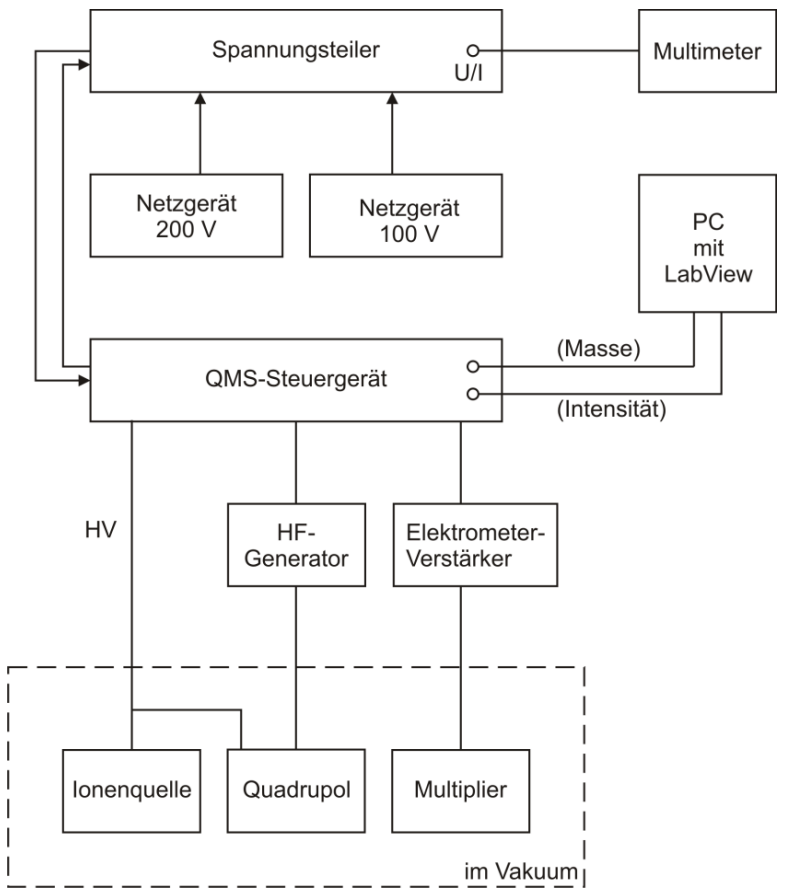
\includegraphics[width=0.85\linewidth]{../resources/figures/schematic_devices.png}
  \caption{Block diagram of the QMS control electronics and data acquisition chain, including RF generation, electrometer readout, and spectrum acquisition on a PC (LabView)~\cite{QMSAnleitung}.}
  \label{fig:setup_electronics}
\end{figure}

Ion creation and injection into the quadrupole are set by the source potentials sketched in Fig.~\ref{fig:setup_potentials}.
A heated filament (cathode, KA) emits electrons by thermionic emission, and the Wehnelt electrode (W) shapes and focuses these electrons into a narrow beam along the source axis.
The electron-impact energy in the formation region (FR) is mainly determined by the potential difference $U_{\mathrm{FR}}-U_{\mathrm{KA}}$, which sets the kinetic energy $E_{\mathrm{EI}}$ of the electrons when they enter FR and thus the ionization conditions.

Positive ions created in the formation region are extracted toward the entrance aperture (Eintrittsblende, EB).
Along this path, the ions are first accelerated out of FR by the potential drop toward the EB region, which helps to pull them out efficiently and form a directed ion beam.
Directly in front of the quadrupole, the ions are then retarded to the field-axis potential $U_{\mathrm{FA}}$, so that their kinetic energy inside the rod system is set mainly by the difference $U_{\mathrm{FR}}-U_{\mathrm{FA}}$.
With the settings used here ($U_{\mathrm{FR}}=113\,\mathrm{V}$, $U_{\mathrm{FA}}=106\,\mathrm{V}$), this corresponds to an injection energy of about $E_{\mathrm{ion}}\approx e\,(U_{\mathrm{FR}}-U_{\mathrm{FA}})\approx 7\,\mathrm{eV}$, which reduces transit speed and improves stable transmission through the quadrupole.

\vspace{1em}
\begin{figure}[H]
  \centering
  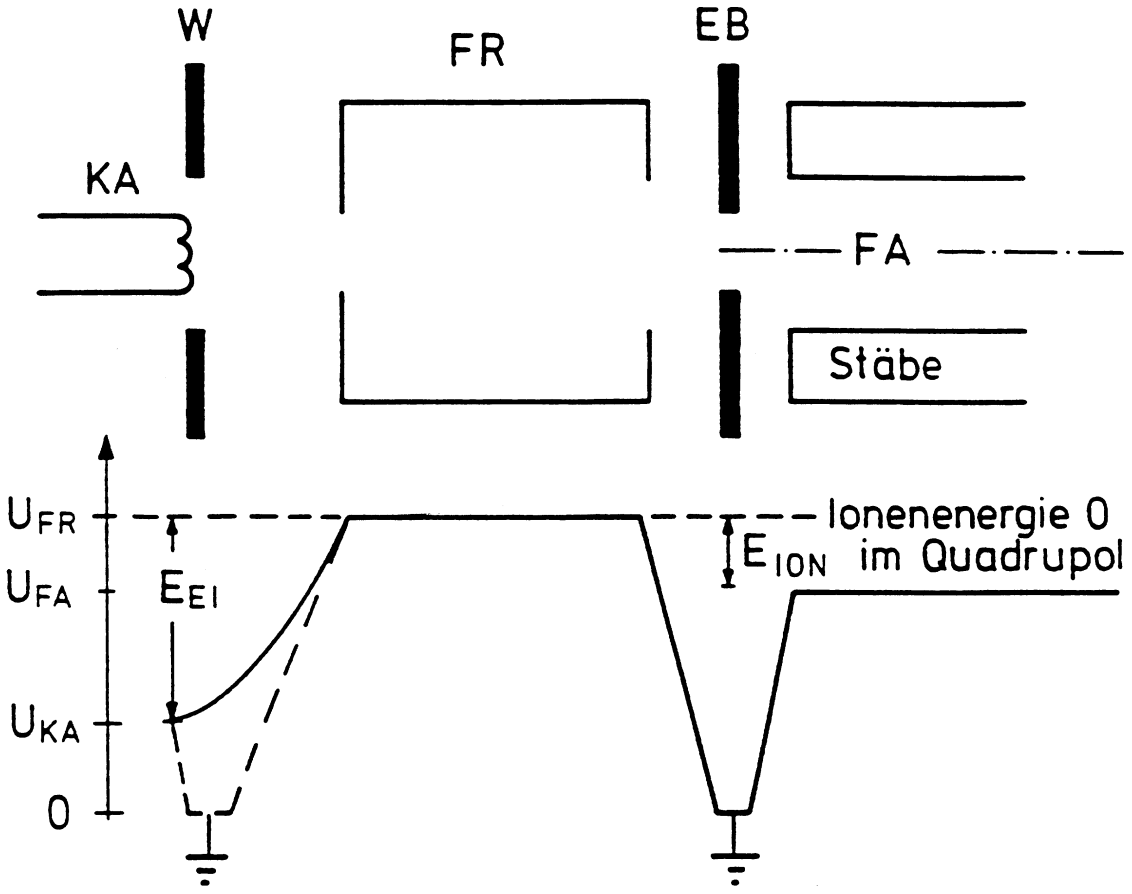
\includegraphics[width=0.98\linewidth]{../resources/figures/schematic_ion_energy.png}
  \caption{Potential/energy scheme of the electron-impact source and injection region.
    Electrons emitted at the cathode (KA) are focused by the Wehnelt electrode (W) and accelerated into the formation region (FR) for ionization.
  The resulting ions are then extracted toward the entrance aperture (EB) and retarded to the field-axis potential $U_{\mathrm{FA}}$ before entering the quadrupole rods~\cite{QMSAnleitung}.}
  \label{fig:setup_potentials}
\end{figure}

% --- Procedure ---
\section{Procedure}

This section summarizes the experimental procedure and relates each step to the measurement tasks defined in the lab script.

\subsection{Pump-down and Instrument Start-up}

The vacuum chamber was evacuated by switching on the (membrane) forepump and subsequently the turbomolecular pump, and the base pressure was reduced to the $10^{-6}\,\mathrm{mbar}$ range.
Before enabling filament emission, the chamber pressure was verified to be below $5\times 10^{-5}\,\mathrm{mbar}$ as required, since at insufficient vacuum the hot cathode can overheat and break (gas cooling is weak and heat removal is mainly by radiation).

The QMS control unit was switched on with emission set to \texttt{OFF}, and the external DC supplies (100 V and 200 V) were enabled.
Emission was then switched to \texttt{ON} and ramped slowly to 0.2 (of the maximum setting 1.0) to reduce thermal stress on the fragile filament during heat-up.
Afterwards, the source potentials were set to $U_{\mathrm{KA}}\approx 0\,\mathrm{V}$ (instrument-limited to $\sim 30\,\mathrm{mV}$), $U_{\mathrm{FR}}=113\,\mathrm{V}$, and $U_{\mathrm{FA}}=106\,\mathrm{V}$.
After filament activation the pressure increased noticeably, and measurements were started only once the pressure had returned close to its previous steady value.
The relevant front-panel controls are shown in Fig.~\ref{fig:qms_control_panels}.

\vspace{1em}
\begin{figure}[H]
  \centering
  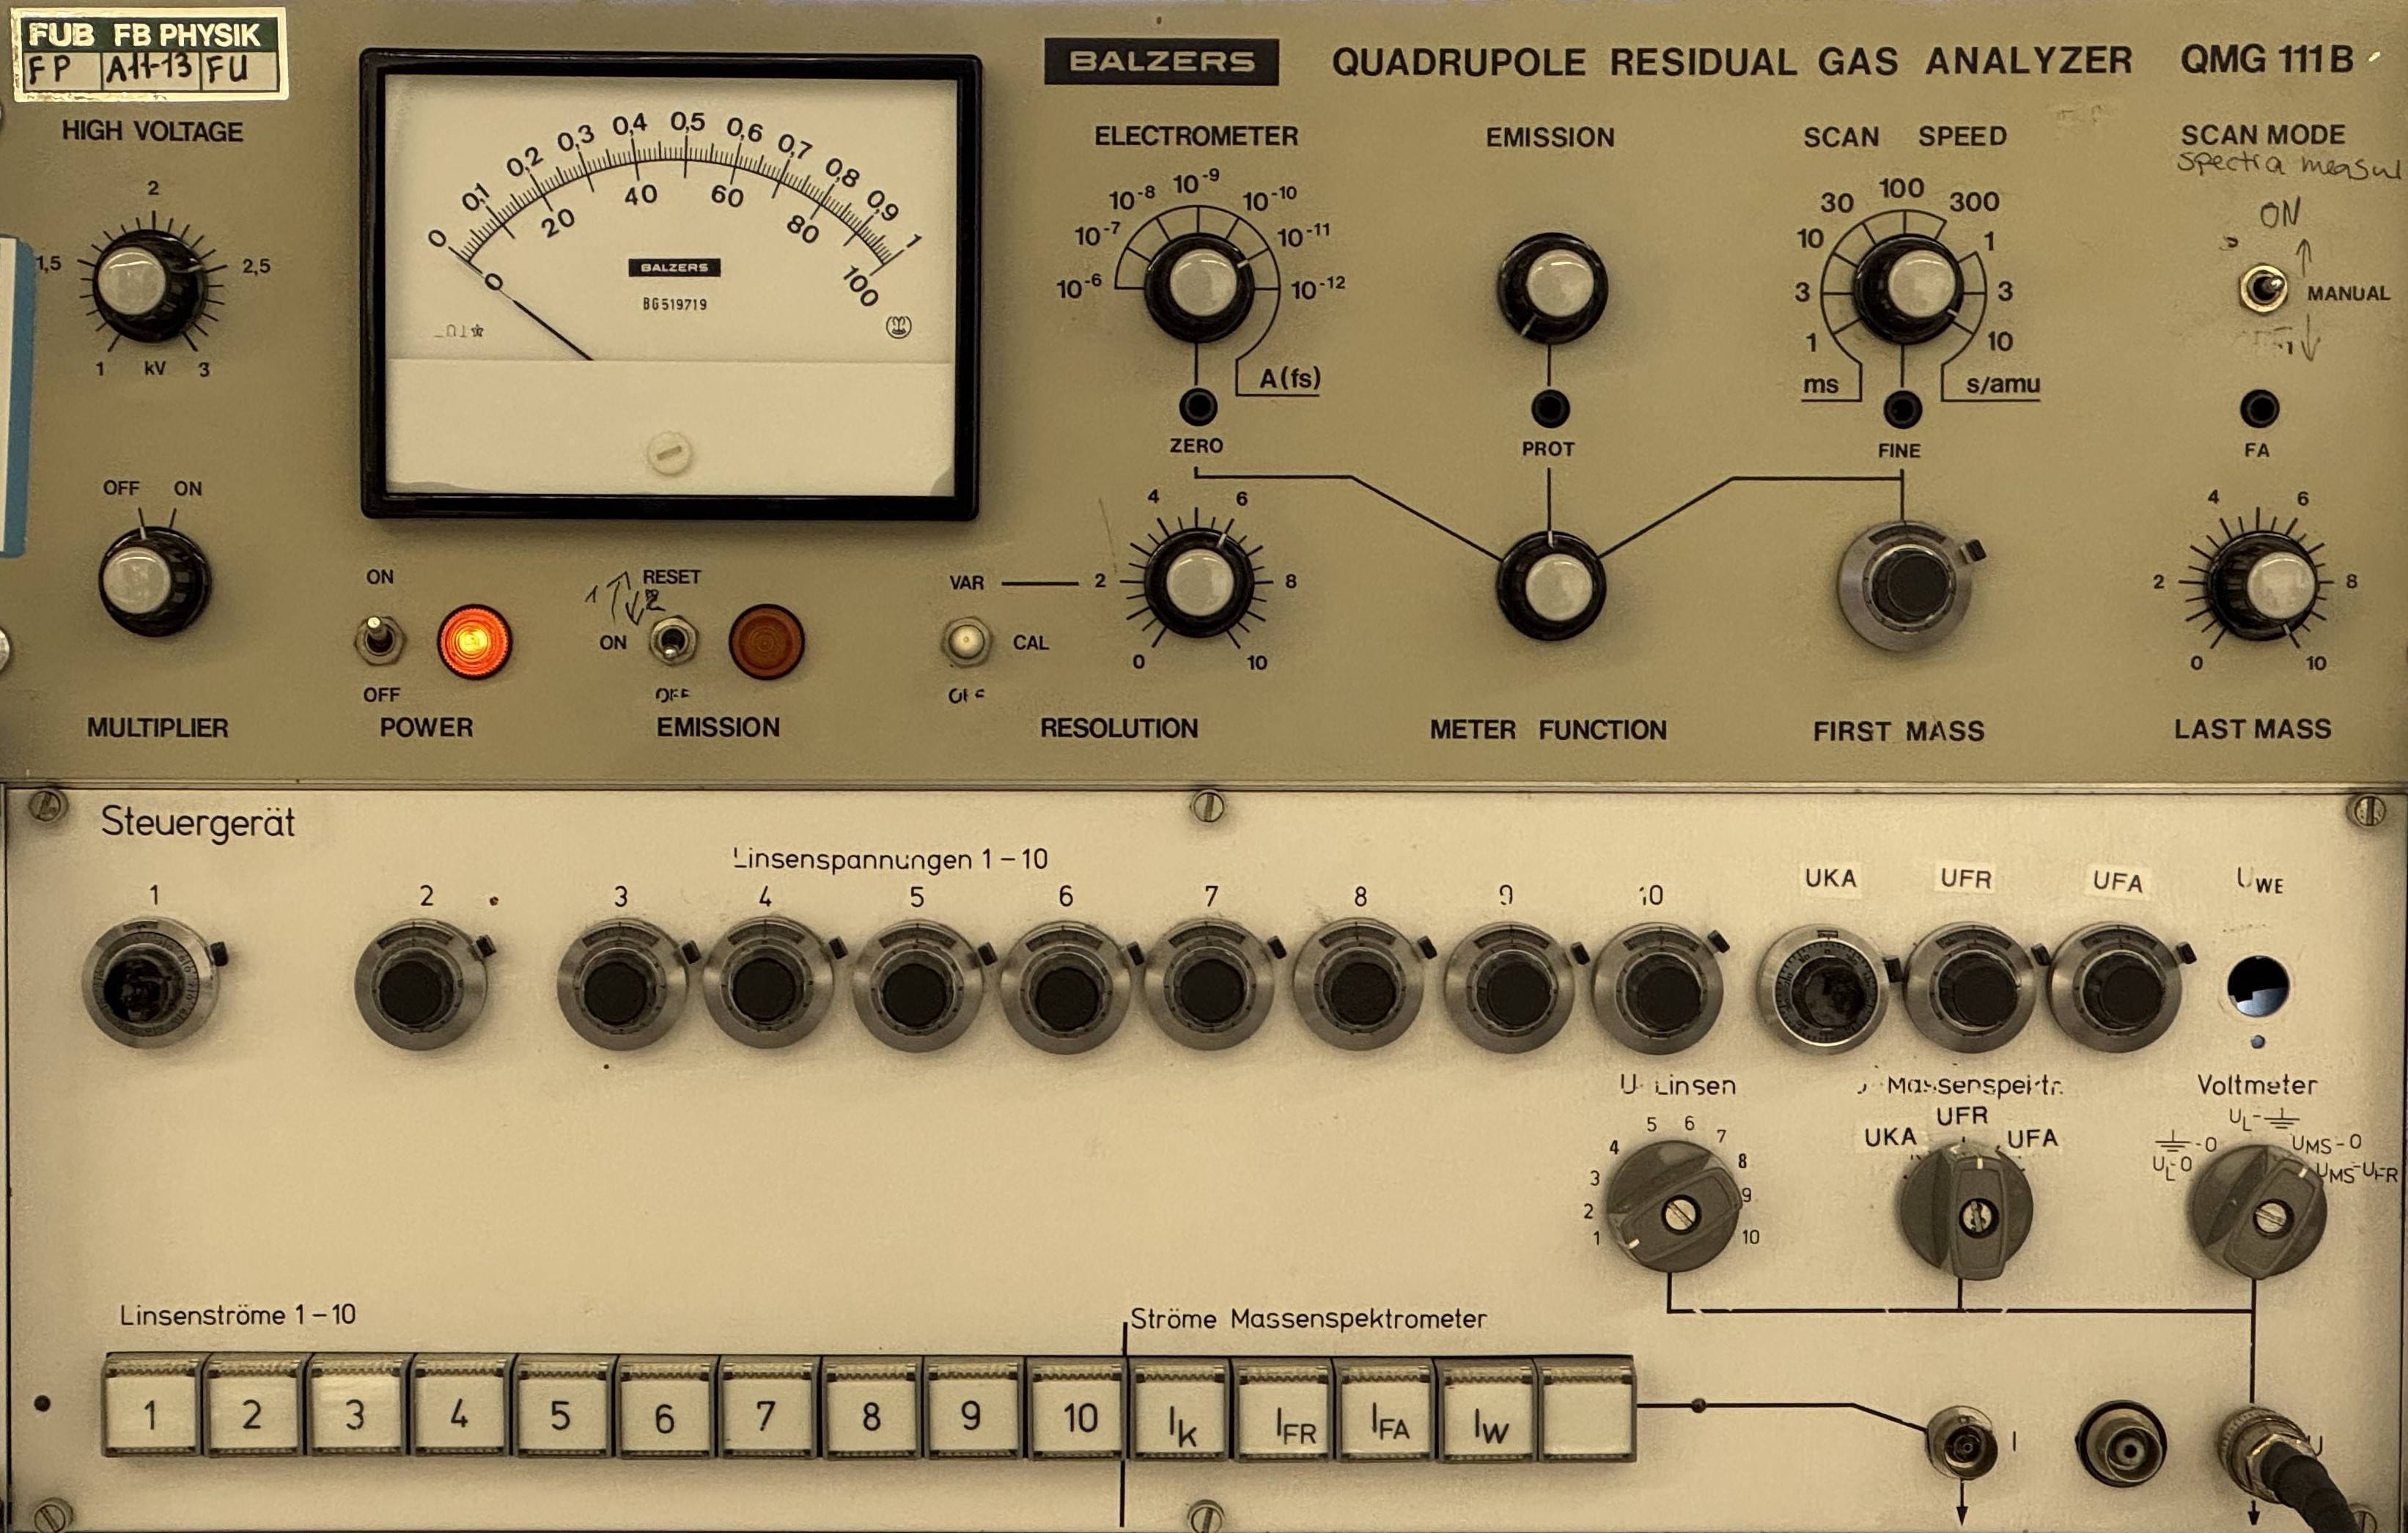
\includegraphics[width=1.0\linewidth]{../resources/figures/qms_control_panels.jpg}
  \caption{Front panels of the QMS electronics used in the experiment.
    Top: Balzers QMG 111B controller with emission control, electrometer range, scan speed and the resolution knob.
    Bottom: auxiliary supply unit providing the adjustable source voltages $(U_{\mathrm{KA}}, U_{\mathrm{FR}}, U_{\mathrm{FA}}$) \\.
  (Own photograph.)}
  \label{fig:qms_control_panels}
\end{figure}

\subsection{Gas-Line Flushing and Gas Dosing}

Mass spectra were recorded for argon, acetone, ethanol, and air, and between different gases the inlet system was flushed to minimize cross-contamination.
For safety and to follow the recommended workflow, emission was switched to \texttt{OFF} whenever a new gas was prepared in the inlet lines.
Flushing was performed with the fine dosing (needle) valve to the chamber kept closed throughout.
First, the selected gas reservoir was opened briefly to fill the first line section.
Then this section was evacuated by opening the valve to the rotary vane pump and closing it again.
Next, the reservoir was opened again briefly, and the second line section up to the dosing valve was flushed by briefly opening the connecting valve between the two line sections, after which it was closed again.
This sequence was repeated for at least three cycles, so that the second line section was left pre-filled with the selected gas before dosing.

For dosing into the chamber, all valves in the inlet system were closed again, in particular the connecting valve between the two line sections, which served as a safety isolation.
The chamber was then dosed only via the fine dosing valve at the recipient inlet, which was opened gradually while pumping continued until the pressure rose to a steady operating value around \(10^{-5}\,\mathrm{mbar}\).
During dosing, care was taken that the pressure did not rise abruptly into the \(10^{-4}\,\mathrm{mbar}\) regime, since excessive pressure can endanger the pumping system and violates the recommended operating limits.
The gas inlet manifold and the two line sections used for flushing and dosing are shown in Fig.~\ref{fig:gas_manifold_photo}.

\vspace{1em}
\begin{figure}[H]
  \centering
  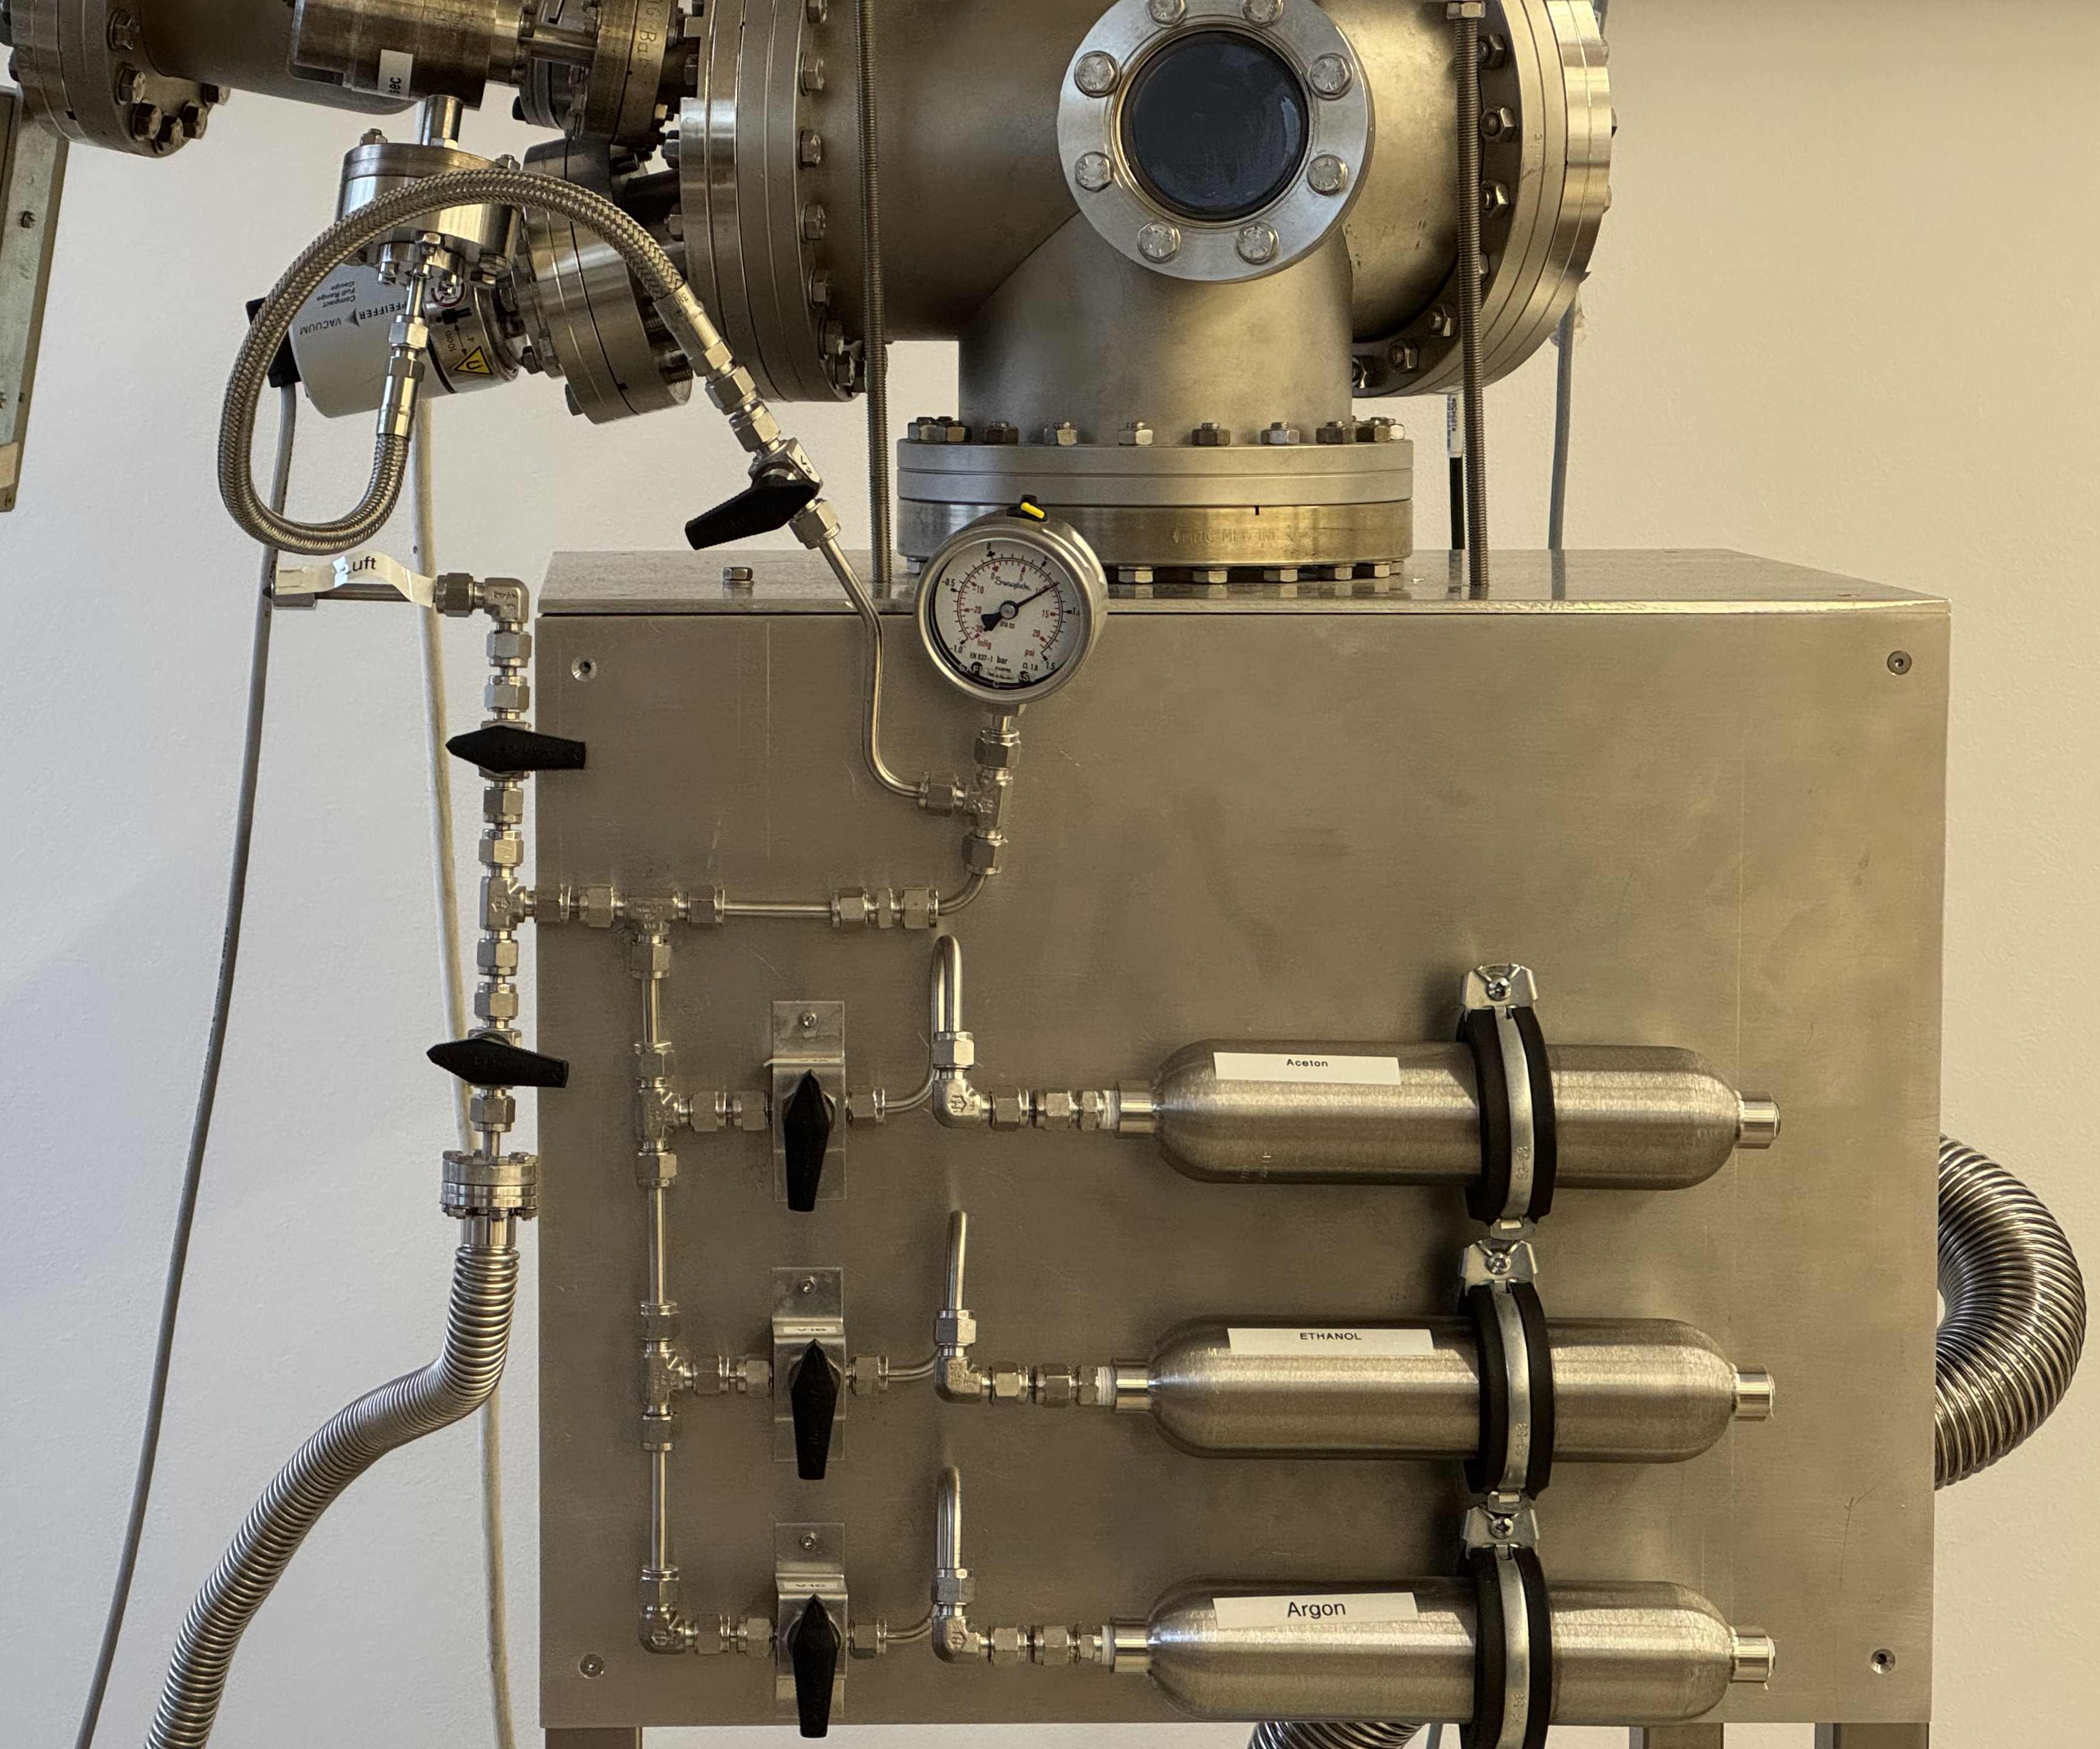
\includegraphics[width=0.95\linewidth]{../resources/figures/gas_manifold.jpg}
  \caption{Gas inlet manifold for flushing and dosing.
    Three reservoirs (acetone, ethanol, argon) and an ambient-air inlet feed into a common manifold with pressure gauge, evacuation connection to a rotary vane pump, and a fine dosing (needle) valve to the recipient.
  (Own photograph.)}
  \label{fig:gas_manifold_photo}
\end{figure}

\subsection{Mass-Spectrum Acquisition and Data Logging}

All spectra were recorded using the LabView acquisition program by scanning the mass range typically from $m/z=4$ to $100$ (amu).
For the final air series (resolution and acceleration-voltage variation), the scan range was reduced to roughly $m/z\approx 4$ to $60$ to focus on the relevant peaks and reduce measurement time.
For each gas, a fast overview scan with $1\,\mathrm{s/amu}$ was recorded first to verify the expected peak pattern and to choose a suitable electrometer range (avoiding saturation while keeping weak peaks visible).
The final spectra were then recorded with $10\,\mathrm{s/amu}$ to improve signal-to-noise.
Electrometer settings were adjusted depending on signal level and were often chosen one decade more sensitive than the recommended values (e.g.\ $10^{-9}$ instead of $10^{-10}$).

At the beginning of the sequence, one background spectrum (residual gas) was recorded at base pressure and used for background subtraction of the argon spectrum.
Due to time constraints, no separate background spectra were recorded for acetone, ethanol, and air, so those spectra were evaluated including the residual-gas contribution.
All spectra were saved as \texttt{.txt} files containing two columns, where the first column is the recorded intensity signal and the second column is the mass channel (stored as $m/10$ by the acquisition software).
Measurement settings and the end-of-scan chamber pressure were encoded in the filenames using the tags \texttt{bg}, \texttt{ar}, \texttt{ac}, \texttt{eth}, \texttt{air}, as well as \texttt{sp} (scan speed), \texttt{em} (electrometer range), \texttt{p} (total pressure), \texttt{res} (resolution), and \texttt{ufa} ($U_{\mathrm{FA}}$).

\subsection{Resolution and Acceleration-Voltage Series in Air}

To determine the resolving power, a series of air spectra was recorded with the resolution setting switched to \texttt{VAR} and stepped through the values 6, 5, 4, 3, and 2 (starting from the highest resolution).
These settings were chosen to match the discrete resolution values used in the provided reference spectra as closely as possible.

To study the influence of ion injection energy, additional air spectra were recorded while varying $U_{\mathrm{FA}}$, which changes the acceleration voltage $U_{\mathrm{B}}=U_{\mathrm{FR}}-U_{\mathrm{FA}}$.
In analogy to the reference series, $U_{\mathrm{FA}}$ was set successively to 112.9\,V, 98.0\,V, 83.0\,V, 63.0\,V, 43.0\,V, 23.0\,V, and 3.0\,V, corresponding to an increasing $U_{\mathrm{B}}$ at fixed $U_{\mathrm{FR}}$.
The sequence was therefore taken from the lowest acceleration voltage (small $U_{\mathrm{B}}$) to the highest (largest $U_{\mathrm{B}}$), while keeping the remaining scan settings fixed.

\subsection{Shutdown}

After completing all measurements, emission was switched to \texttt{OFF} first, then the external voltage supplies were switched off, and finally the QMS control unit was turned off, following the recommended shutdown order.

% --- Results ---
\section{Results}
\subsection{Argon Spectrum}
A measurement of the background spectrum was recorded to implement a background subtraction to the recorded spectrum of the ionized Argon. First, both spectrum were normalized by pressure and then the background spectrum was subtracted from the Argon spectrum (Figure~\ref{fig:argon}). The effect of the substraction is substantially noticeable in the $H_2O^+$ peak ($18Th$). We can appreciate potential impurities around the $28Th$ range, attributed to $N_2^+$. The comparison to the reference spectrum confirms the expected peaks found in our data (Figure~\ref{fig:argon-reference}).

\begin{figure}[htbp]
  \centering
  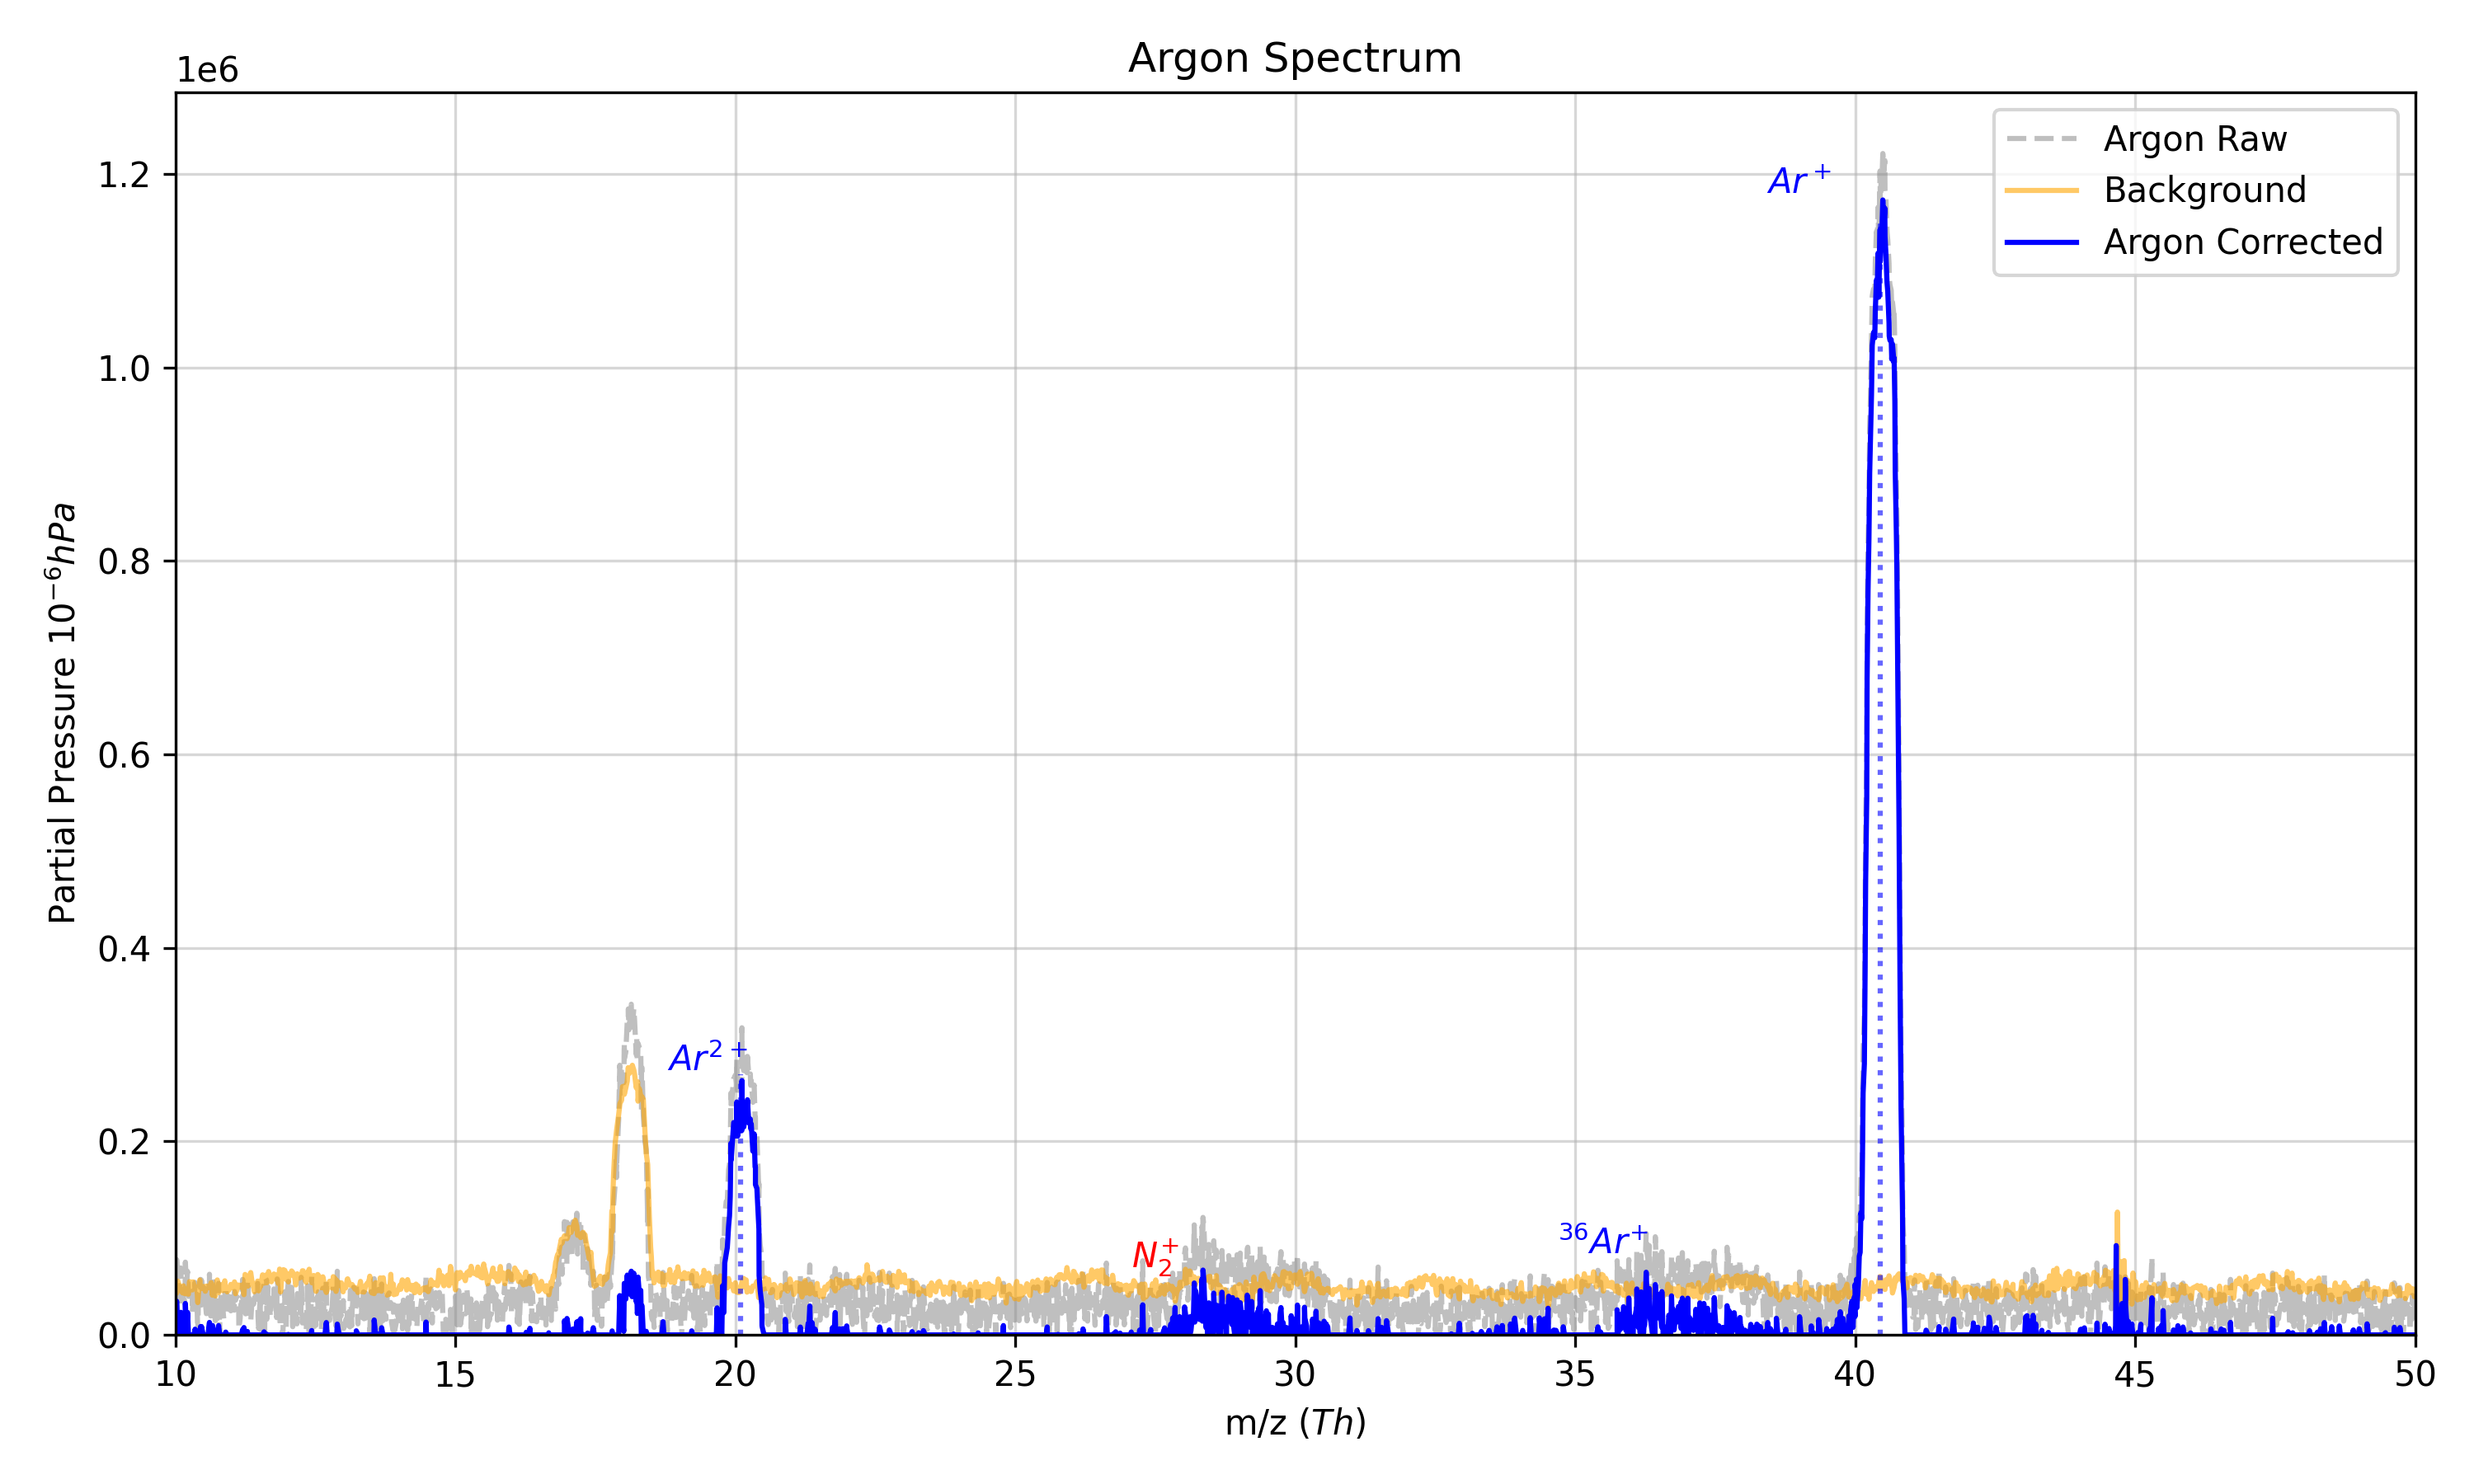
\includegraphics[width=0.9\linewidth]{../resources/task_5_1_argon.png}
  \caption{Corrected Argon spectrum, background spectrum, and recorded background spectrum. The intensities were normalized according to their respective pressure values and the spectrums were matched using the $H_2O^+$ peak as reference.}\label{fig:argon}
\end{figure}

\begin{figure}[htbp]
  \centering
  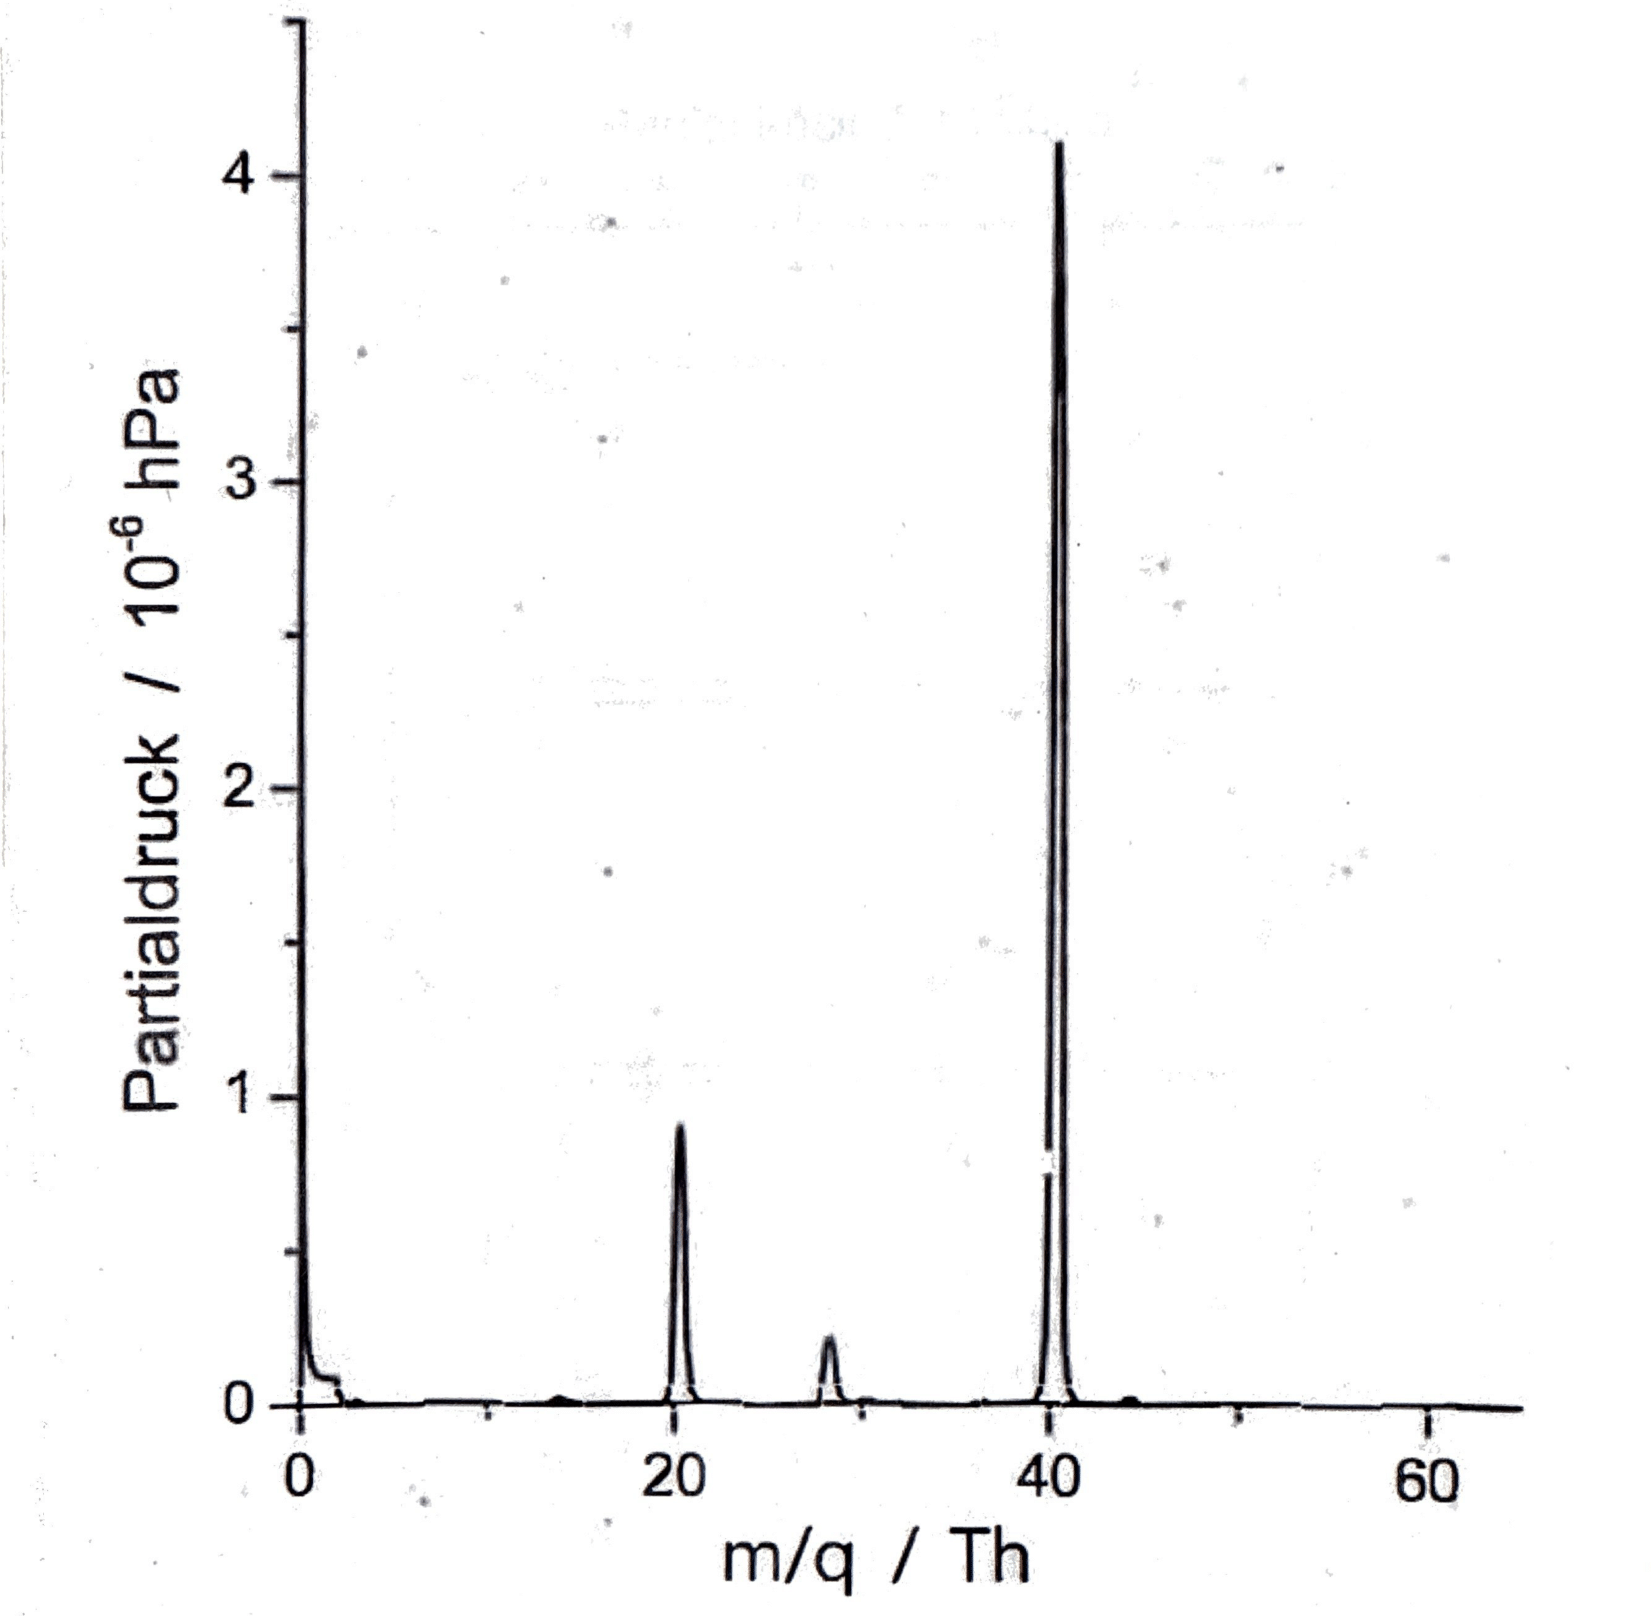
\includegraphics[width=0.6\linewidth]{../resources/figures/QMS_Beispiel-Spektren/QMS_Beispiel-Spektren-2.png}
  \caption{Reference spectrum for Argon.}\label{fig:argon-reference}
\end{figure}

\subsection{Acetone Spectrum}
Figure~\ref{fig:acetone} contains the acetone spectrum in the range of 10 to 60$Th$, with normalized pressure. The dominant peaks (blue), fragment peaks (gray), and impurities (red) were labelled in the plot. The comparison to the reference spectrum confirms the expected peaks found in our data (Figure~\ref{fig:acetone-reference}).

\begin{figure}[htbp]
  \centering
  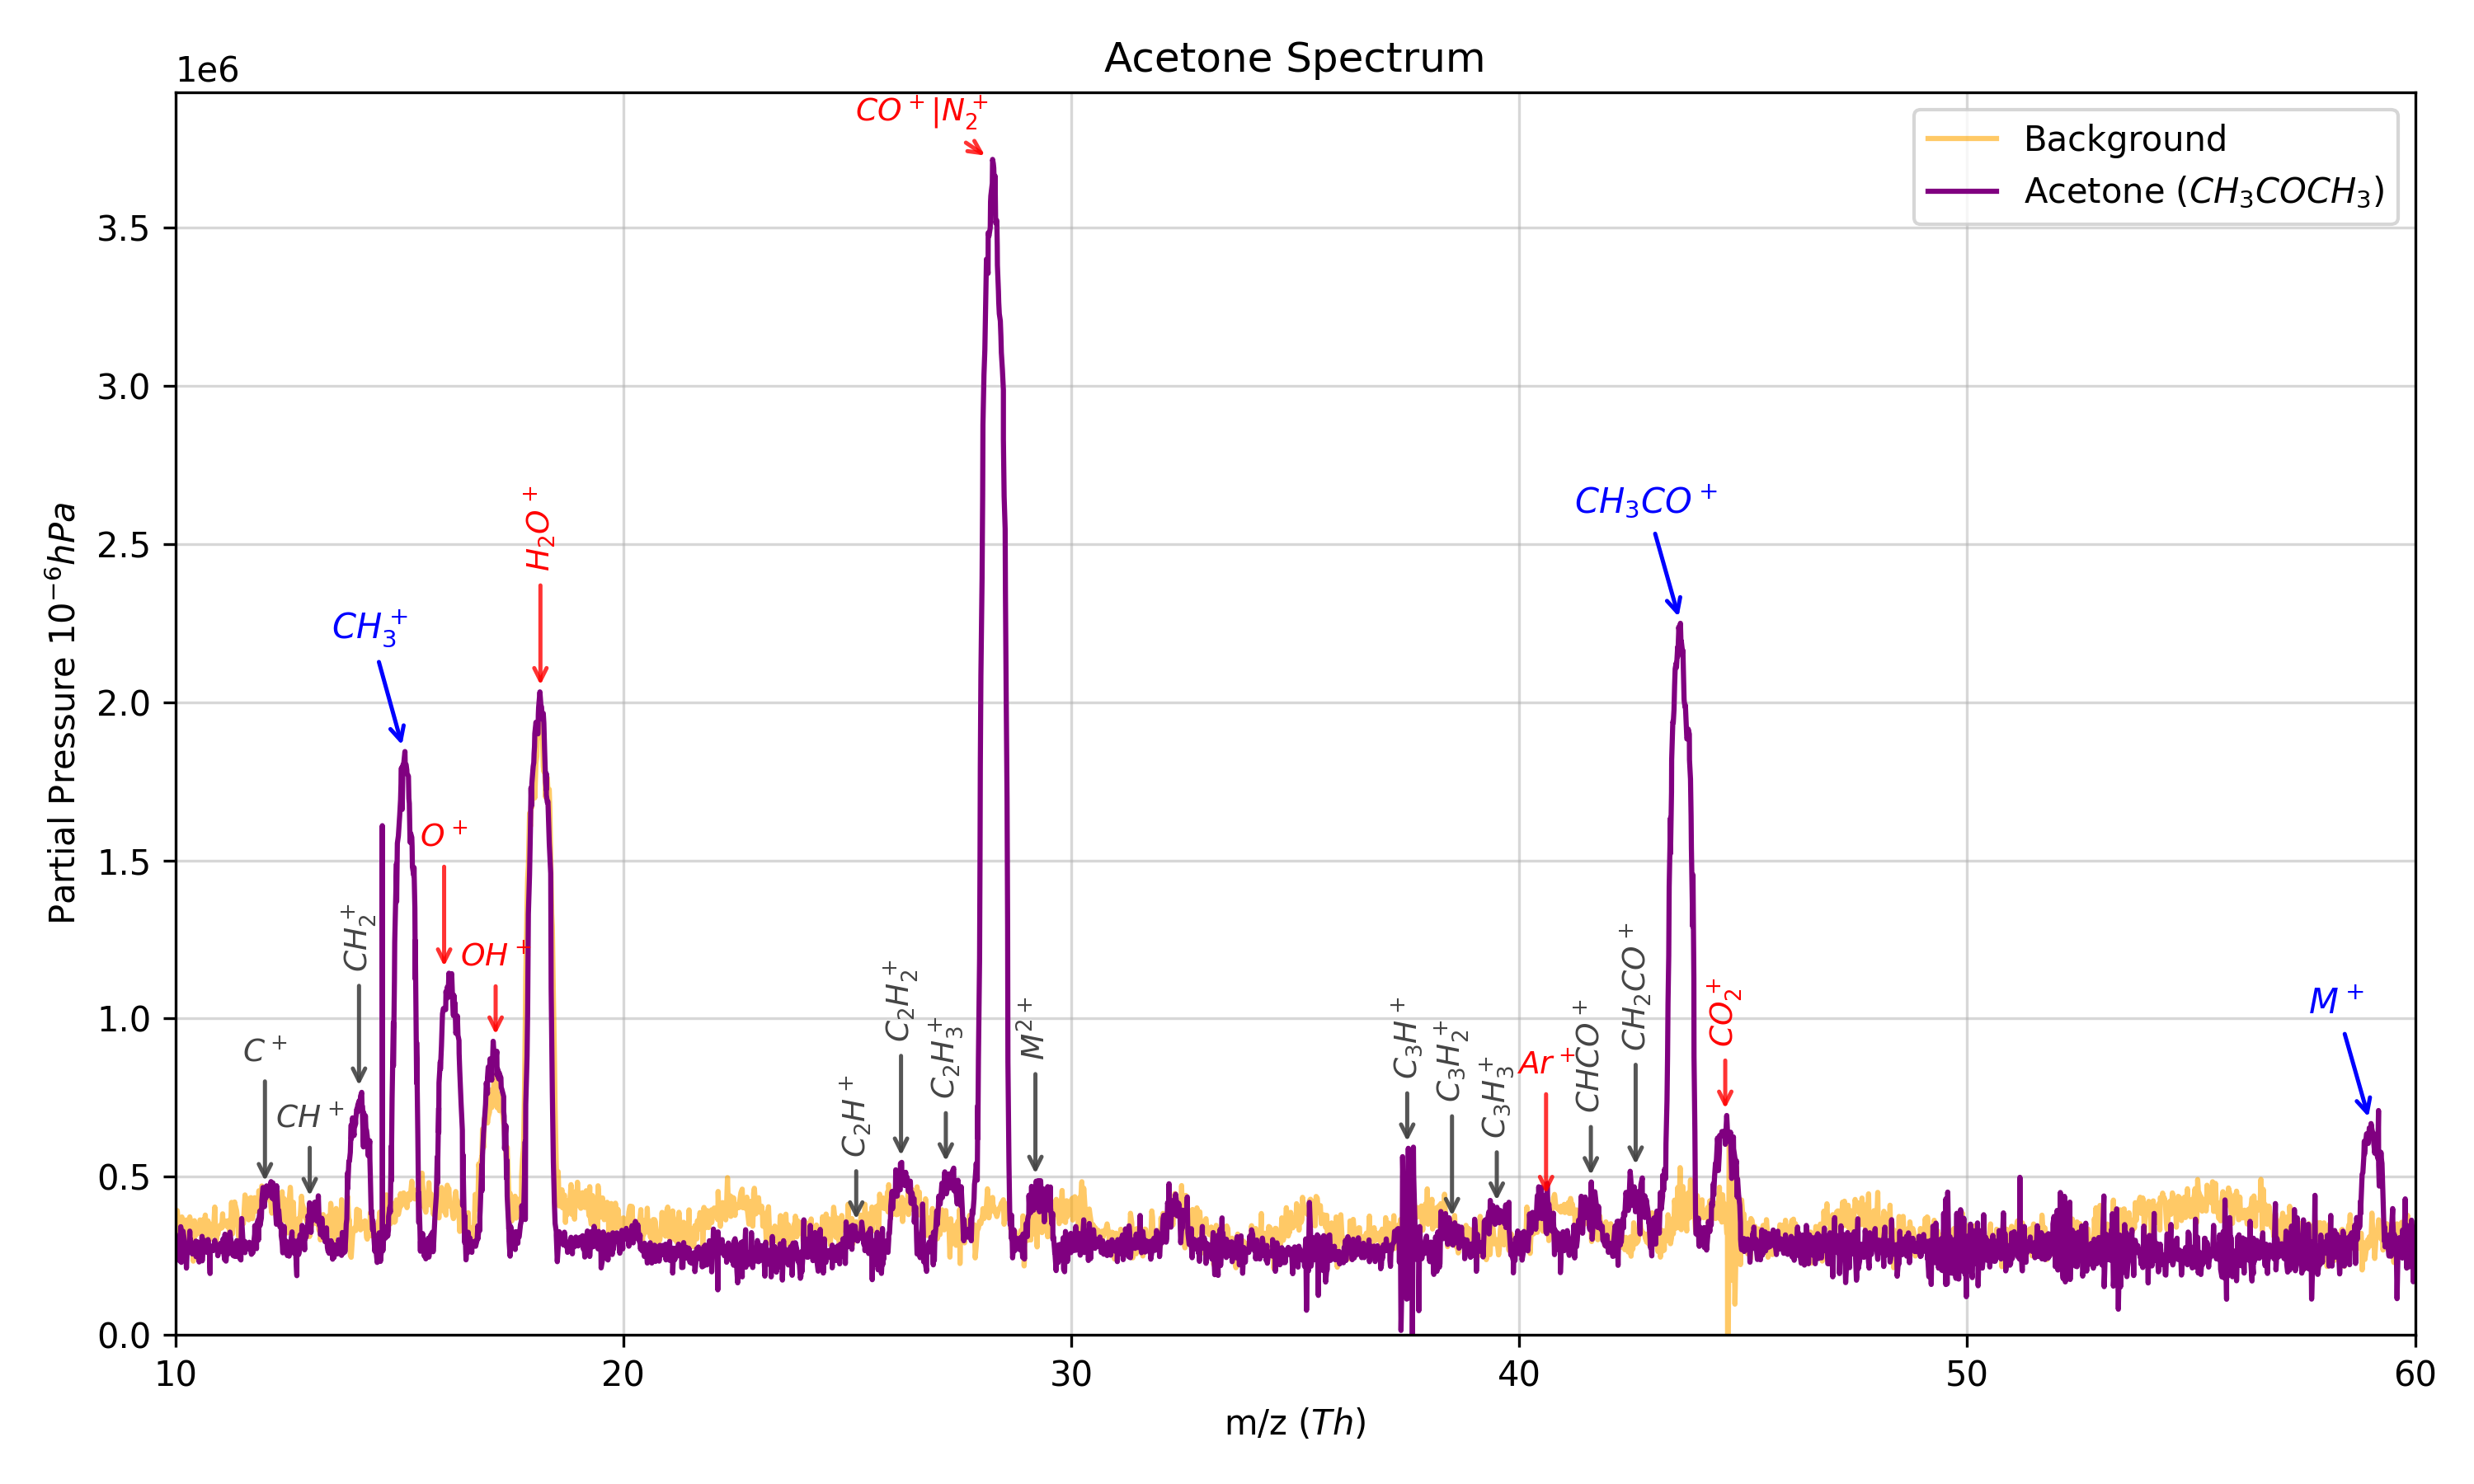
\includegraphics[width=0.9\linewidth]{../resources/task_5_2_acetone.png}
  \caption{Mass-to-charge spectrum of the recorded measurement for the Acetone sample with normalized pressure.}\label{fig:acetone}
\end{figure}

\begin{figure}[htbp]
  \centering
  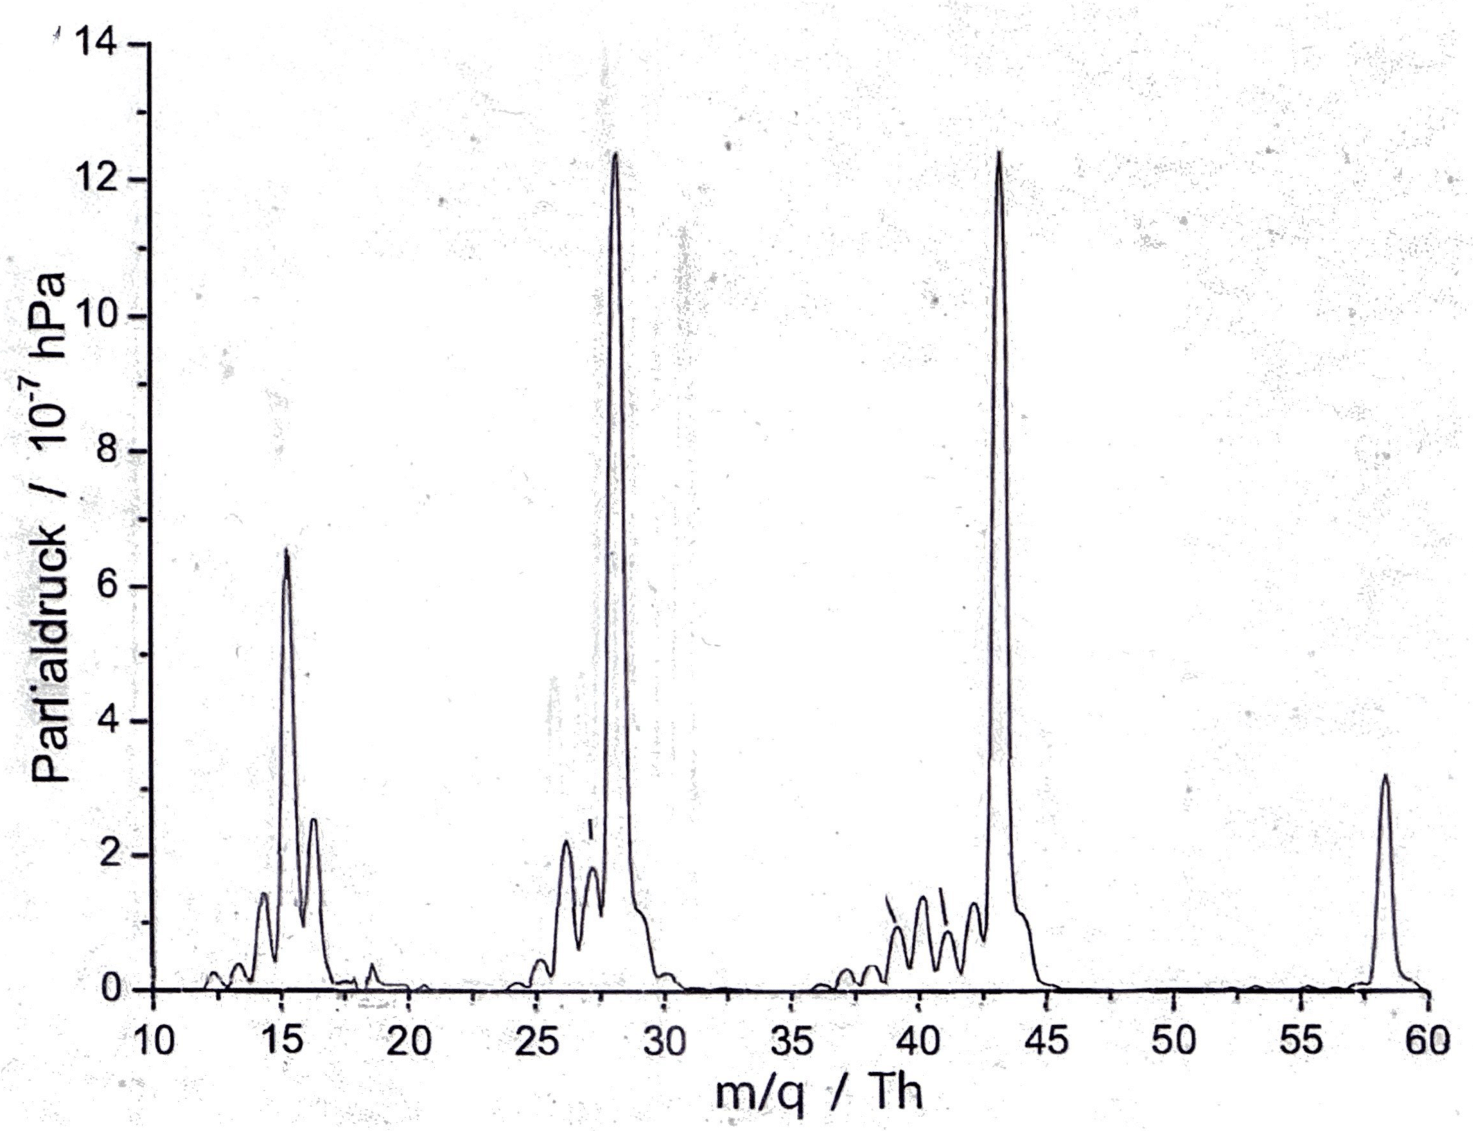
\includegraphics[width=0.8\linewidth]{../resources/figures/QMS_Beispiel-Spektren/QMS_Beispiel-Spektren-3.png}
  \caption{Reference spectrum for Acetone.}\label{fig:acetone-reference}
\end{figure}

\subsection{Ethanol Spectrum}
Figure~\ref{fig:ethanol} contains the ethanol spectrum in the range of 10 to 50Th, with normalized pressure. The dominant peaks (blue), fragment peaks (gray), and impurities (red) were labelled in the plot. The comparison to the reference spectrum again confirms the expected peaks found in our data (Figure~\ref{fig:ethanol-reference}).

\begin{figure}[htbp]
  \centering
  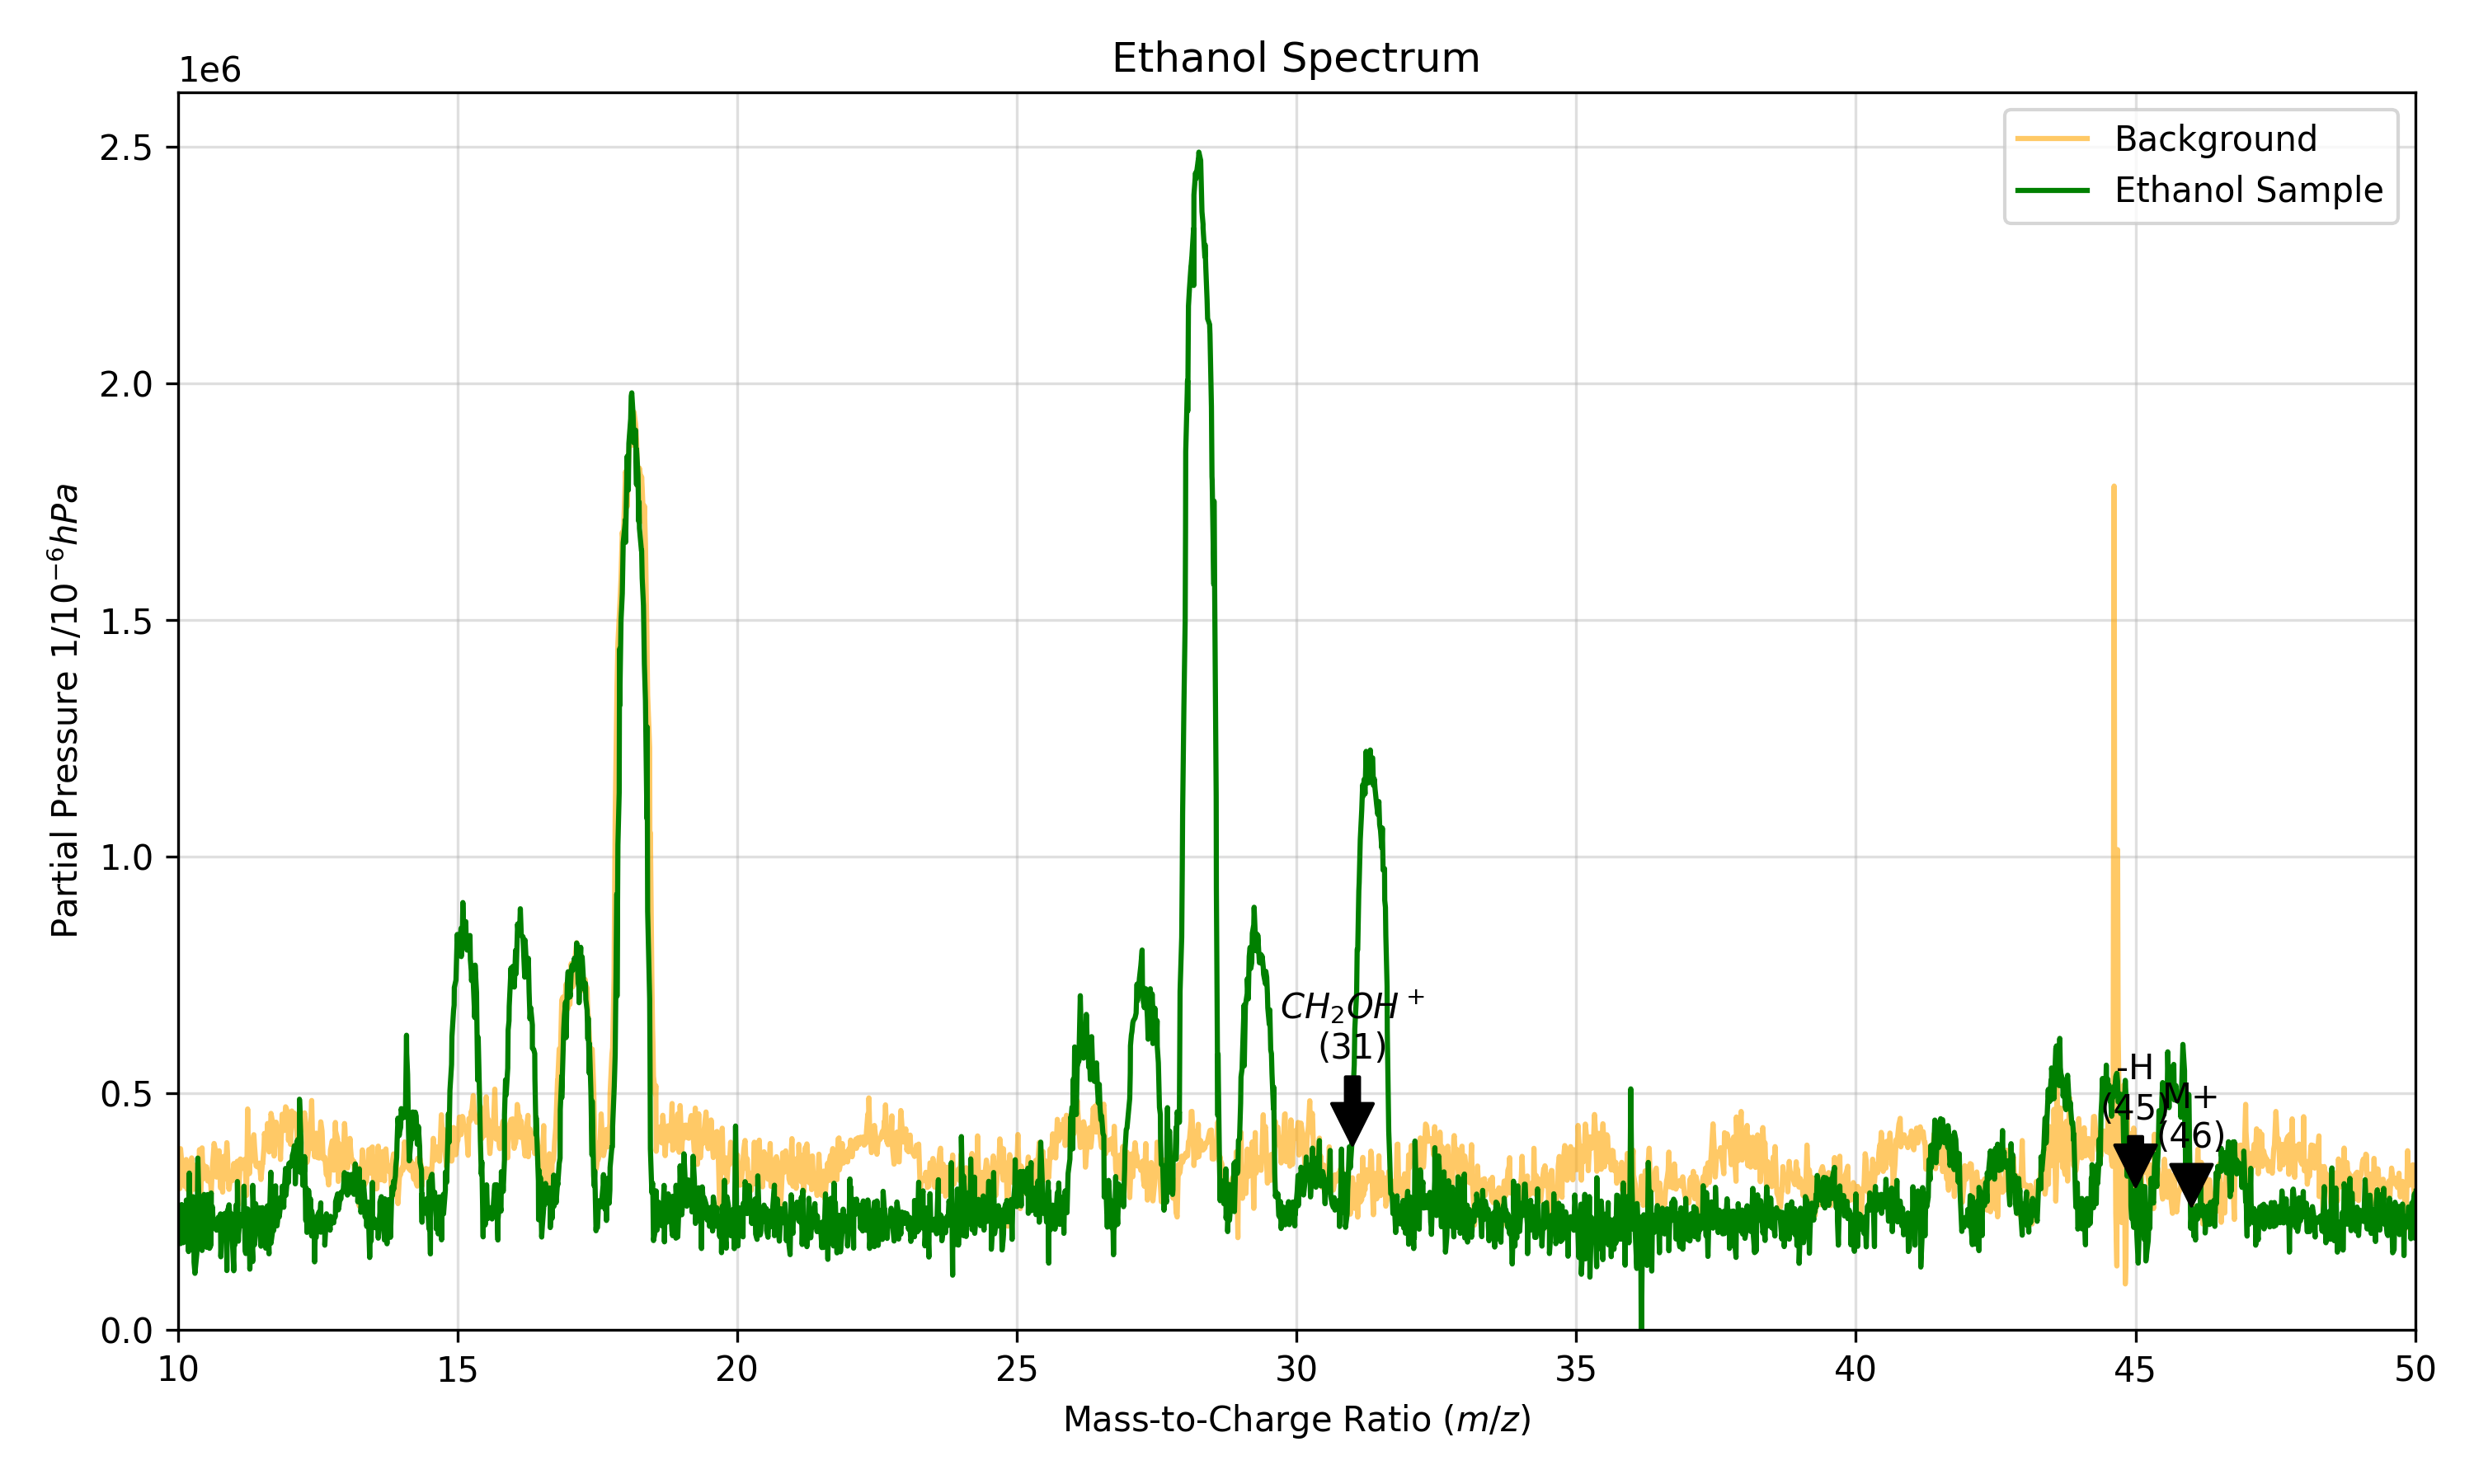
\includegraphics[width=0.9\linewidth]{../resources/task_5_3_ethanol.png}
  \caption{Mass-to-charge spectrum of the recorded measurement for the Ethanol sample with normalized pressure.}\label{fig:ethanol}
\end{figure}

\begin{figure}[htbp]
  \centering
  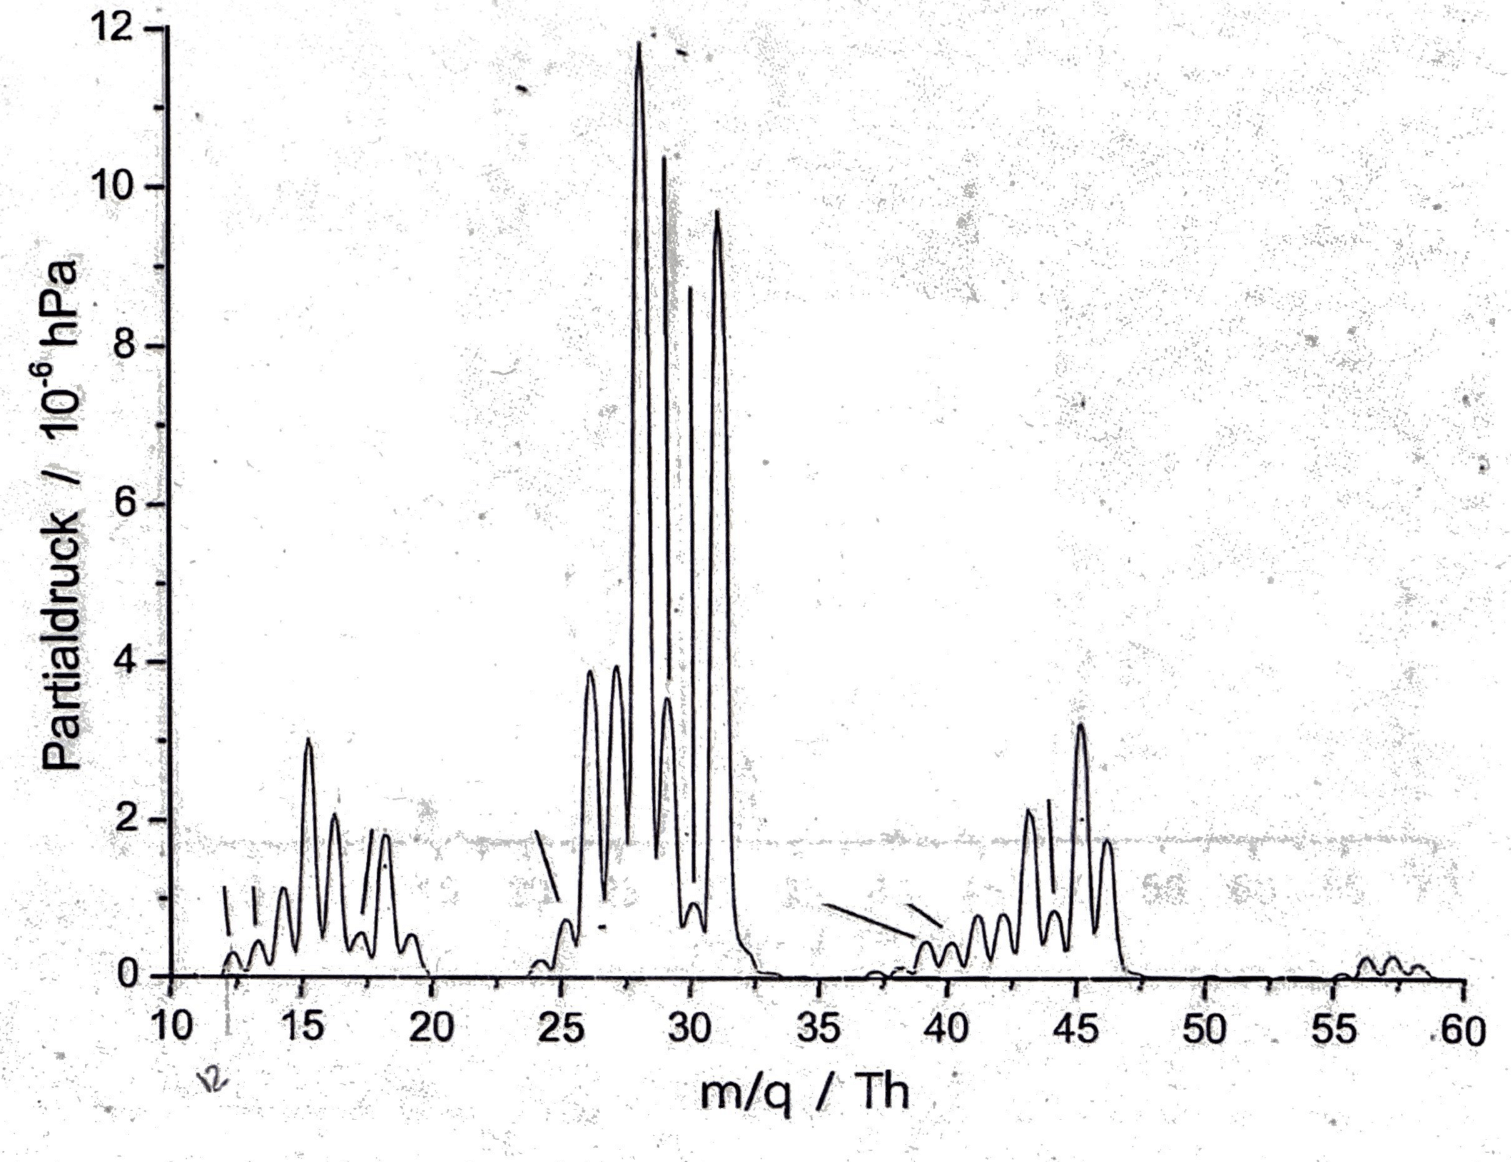
\includegraphics[width=0.8\linewidth]{../resources/figures/QMS_Beispiel-Spektren/QMS_Beispiel-Spektren-4.png}
  \caption{Reference spectrum for Ethanol.}\label{fig:ethanol-reference}
\end{figure}

\subsection{Air Spectrum}
Figure~\ref{fig:air} contains the air spectrum in the range of 10 to 50$Th$, with normalized pressure. The dominant peaks (blue), and impurities (red) were labelled in the plot. Unfortunately the comparison to the reference spectrum again shows that we are missing in our data both the $Ar^+$ peak at $40Th$ and the impurity peak from $CO_2^+$ at $44Th$(Figure~\ref{fig:air-reference}).

\begin{figure}[htbp]
  \centering
  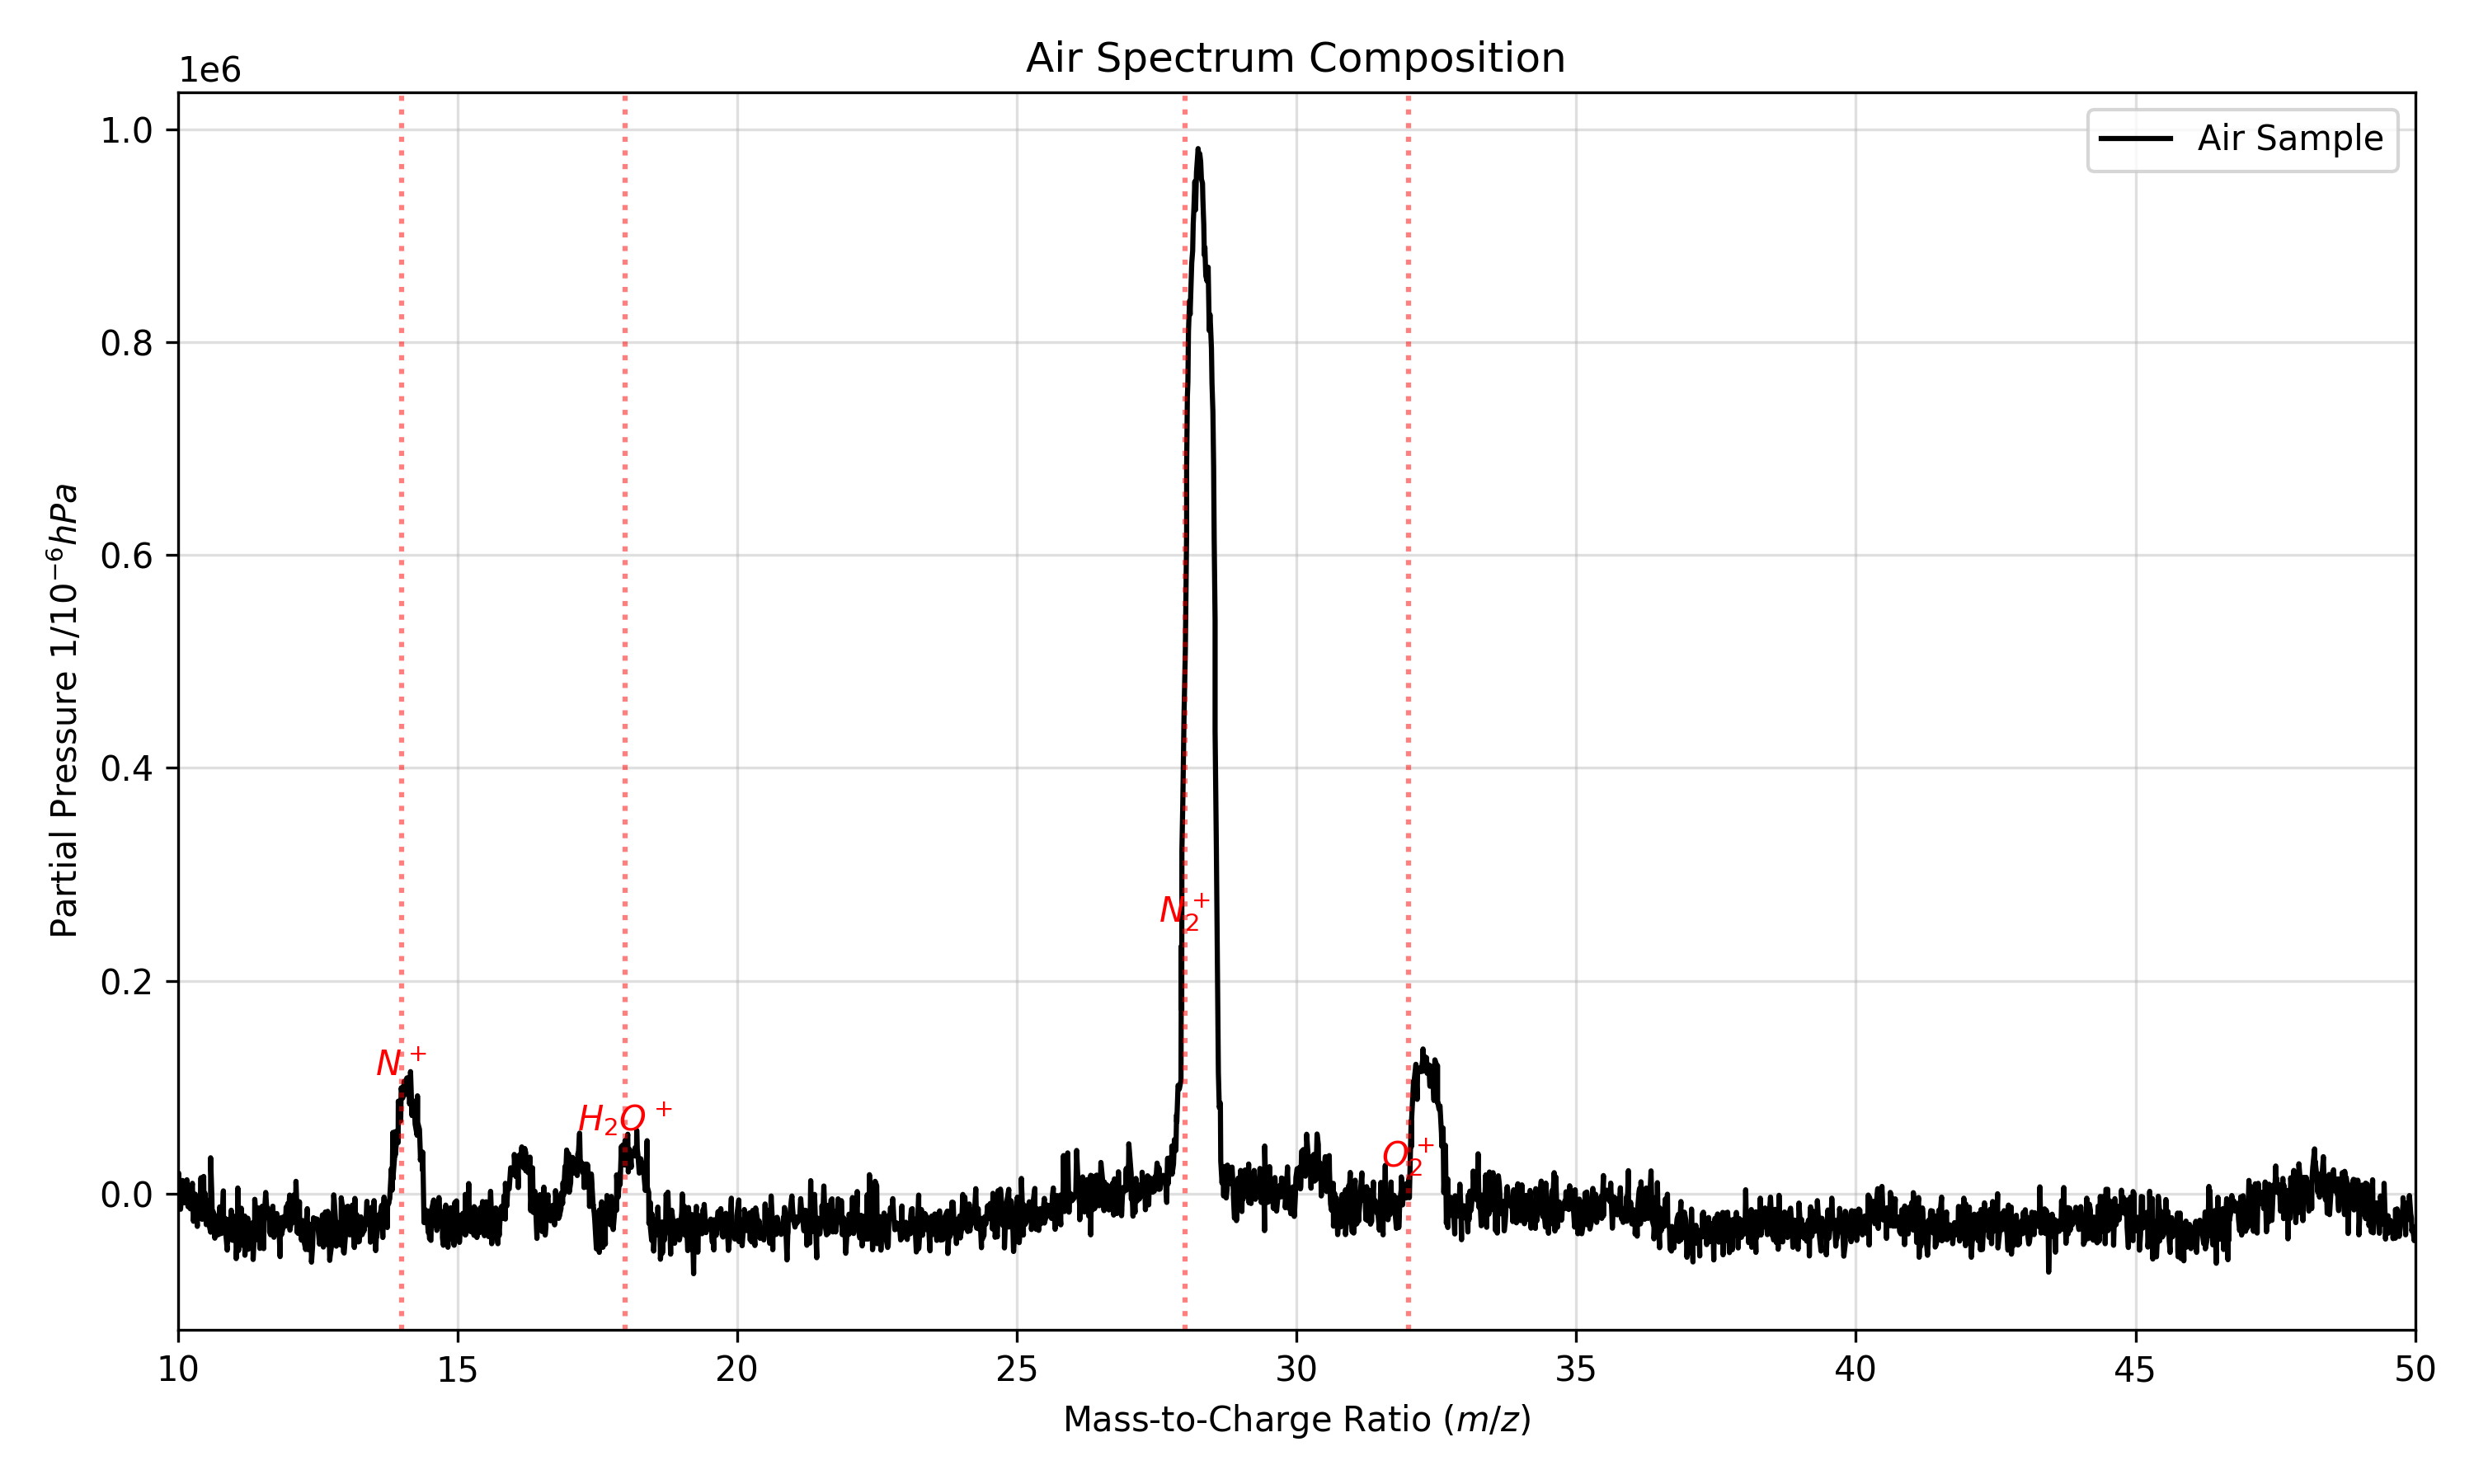
\includegraphics[width=0.9\linewidth]{../resources/task_5_4_air.png}
  \caption{Mass-to-charge spectrum of the recorded measurement for the air composition with normalized pressure.}\label{fig:air}
\end{figure}

\begin{figure}[htbp]
  \centering
  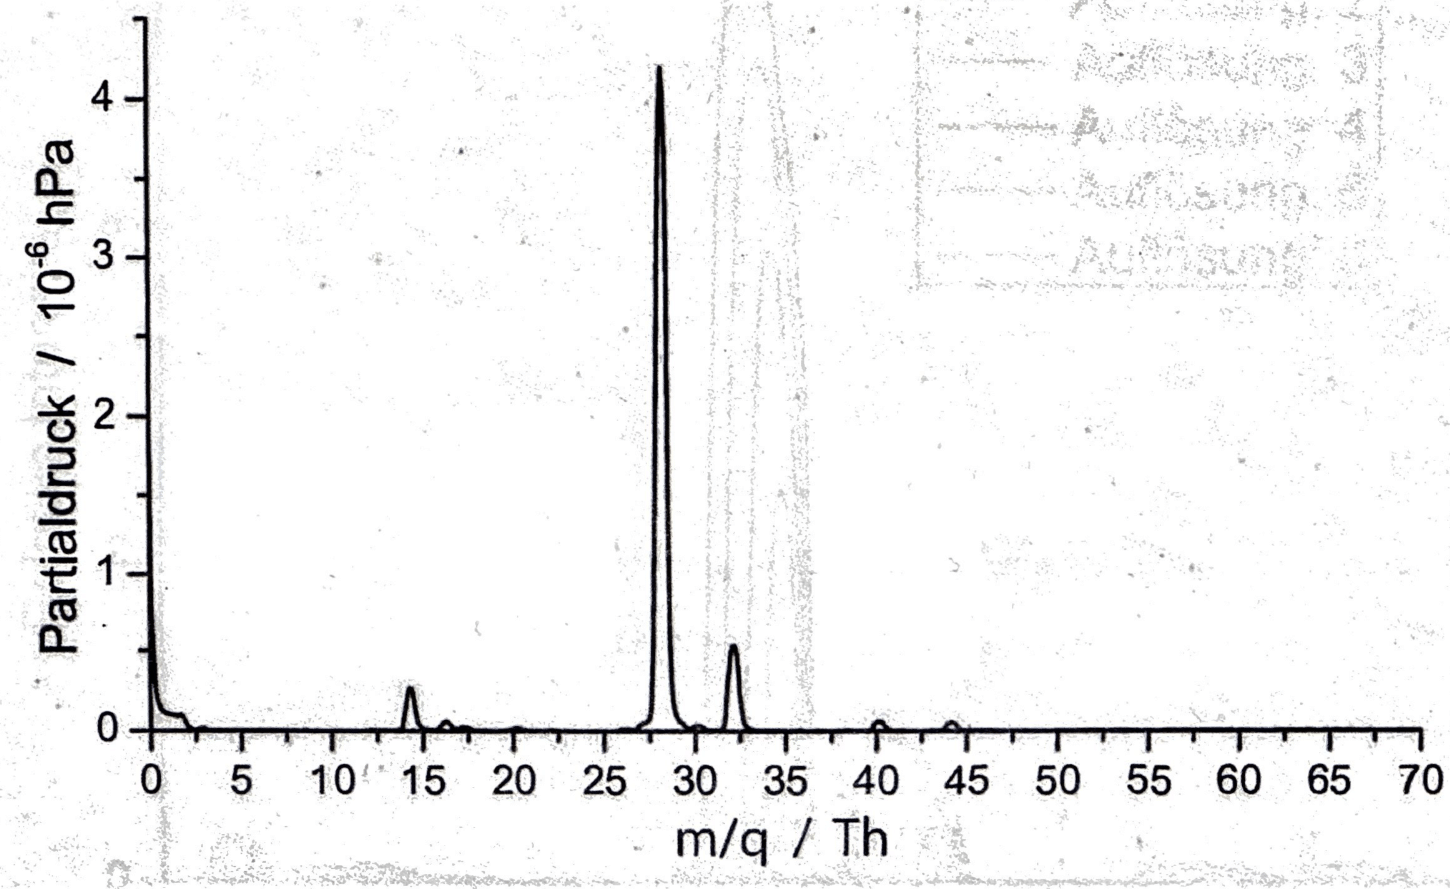
\includegraphics[width=0.8\linewidth]{../resources/figures/QMS_Beispiel-Spektren/QMS_Beispiel-Spektren-5.png}
  \caption{Reference spectrum for air.}\label{fig:air-reference}
\end{figure}

\subsection{Resolution Analysis}
\subsubsection{Introduction}
As discussed previously in Section~\ref{sec:working_line}, the working line always intersects the edge of the stability region at the same boundary points $(a_1,b_1)$ and $(a_2,b_2)$, with $b_0/\Delta b=const$. The value $b_0=0.706$ is derived from the solutions to the Mathieu Equations.

Since $m(b)=\frac{2QV}{r_0^2\omega^2b}$, then
\begin{equation}
  \frac{m(b_0)}{\Delta m}=\frac{1/b_0}{1/b_2-1/b_1}=R=const
\end{equation}

It is also important to consider the $U/V$ ratio limit of

\begin{equation}
  \frac{U}{V}<0.1678
\end{equation}

Since $R$ remains constant, changing the $U/V$ ratio allows the user to set a specific resolution that remains consistent across the entire mass spectrum.

\subsubsection{Comparison of Resolution Spectrum}
The mass-to-charge spectrum of air was analyzed using five different resolution settings. An overlay of the five spectrums is shown in Figure~\ref{fig:resolution}

\begin{figure}[htbp]
  \centering
  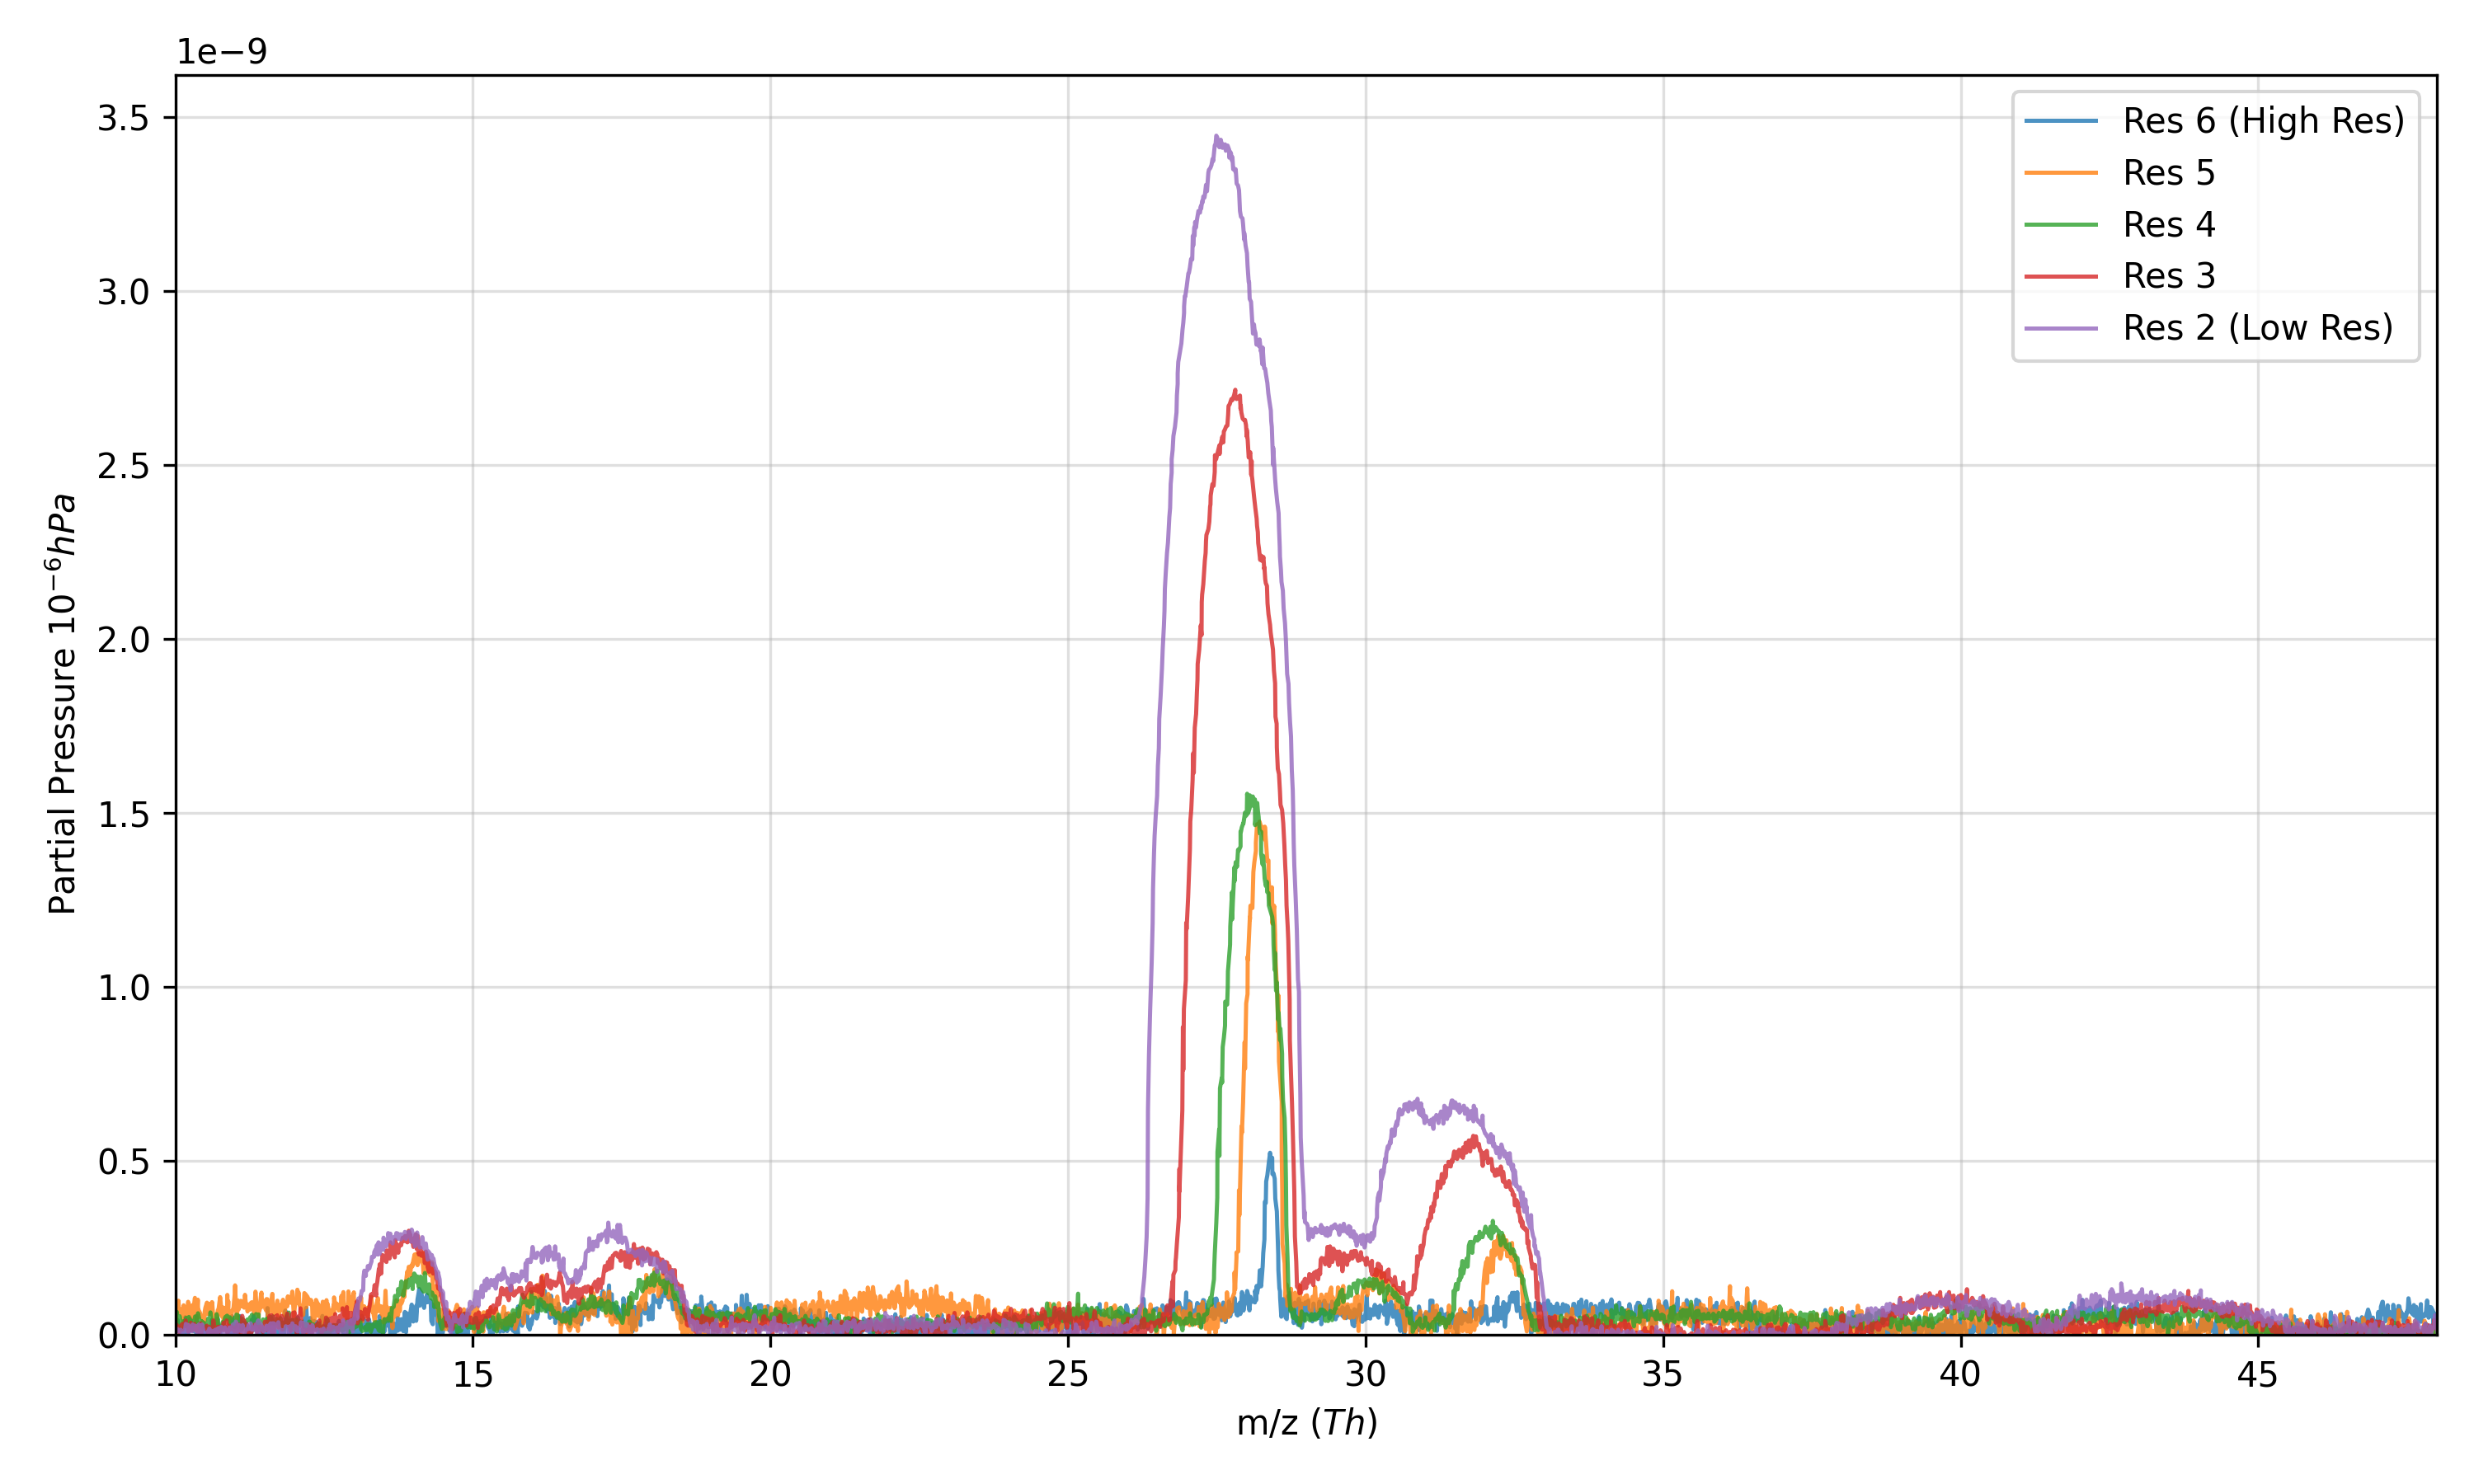
\includegraphics[width=0.9\linewidth]{../resources/task_5_5_resolution_overlay.png}
  \caption{Comparison of the air mass-to-charge spectrumfor differnet resolution values.}\label{fig:resolution}
\end{figure}

\begin{table}[ht]
  \centering
  \resizebox{\textwidth}{!}{
    \begin{tabular}{l|c|cc|cc|cc|cc|cc}
      \toprule
      \textbf{Peak} & \textbf{Mass}& \multicolumn{2}{c|}{\textbf{Res 6}} & \multicolumn{2}{c|}{\textbf{Res 5}} & \multicolumn{2}{c|}{\textbf{Res 4}} & \multicolumn{2}{c|}{\textbf{Res 3}} & \multicolumn{2}{c}{\textbf{Res 2}} \\
      & $m$ [amu] & $\Delta m$ [Th] & $R$ & $\Delta m$ [Th] & $R$ & $\Delta m$ [Th] & $R$ & $\Delta m$ [Th] & $R$ & $\Delta m$ [Th] & $R$ \\
      \midrule
      $N^{+}$    & 14 & 0.2481 & 56.83 & 0.4759 & 29.78 & 0.6712 & 21.14 & 0.9961 & 13.98 & 1.2838 & 10.88 \\
      $H_2O^{+}$ & 18 & 0.2147 & 85.35 & 0.5131 & 35.19 & 0.6401 & 28.28 & 1.3820 & 12.81 & 1.5521 & 11.13 \\
      $N_2^{+}$  & 28 & 0.2253 & 126.03 & 0.6113 & 46.16 & 1.0031 & 27.92 & 1.5824 & 17.57 & 2.2132 & 12.42 \\
      $O_2^{+}$  & 32 & 0.2468 & 131.87 & 0.6598 & 48.85 & 1.0130 & 31.72 & 1.7287 & 18.40 & 2.5702 & 12.01 \\
      $Ar^{+}$   & 40 & 0.0341 & 1139.64 & 0.0498 & 824.39 & 0.3106 & 128.50 & 1.4243 & 28.16 & 1.0973 & 36.24 \\
      \bottomrule
    \end{tabular}
  }
  \caption{FWHM ($\Delta m$) and Resolving Power ($R$) for Air Peaks across Resolution Settings.}\label{tab:fwhm_results}
\end{table}

\begin{itemize}
  \item Plot $m$ versus $\Delta m$ as requested and extract/compare resolving power trends
\end{itemize}

\subsection{Acceleration-Voltage Series in Air (Variation of \texorpdfstring{$U_\mathrm{FA}$}{})}

\begin{itemize}
  \item Overlay the air spectra for the used $U_\mathrm{FA}$ values (112.9, 98.0, 83.0, 63.0, 43.0, 23.0, 3.0 V) and compute $U_\mathrm{B}=U_\mathrm{FR}-U_\mathrm{FA}$ for each case
  \item For two chosen masses, extract $\Delta m$ (FWHM) at each $U_\mathrm{B}$
  \item Convert each setting to an ion oscillation count in the rods using the given rod length $l=0.1$ m and RF frequency $\nu=2.5$ MHz, then plot $\Delta m$ versus number of oscillations for both masses
\end{itemize}

% --- Discussion ---
\section{Discussion}

\subsection{xxx}

Task 1: Comment that the effect of the substraction is substantially noticeable in the H2O+ peak. Talk about the N2 and 36m/z range.
Task 2 to 4: Compare to the references spectrums and discuss unexpected peaks or overlaps (e.g. air/water background, argon remnants). Talk extensively of the peaks and structure of each molecule please.
Task 5: discuss the qualitative trade-off (peak narrowing vs signal loss)

% --- Conclusion ---
\section{Conclusion}

xxx

% --- Appendix ---
\newpage
\section{Appendix}

Additional files:

\begin{itemize}
  \item \texttt{'QMS\_Python.zip'}
  \item \texttt{'QMS\_LabReport.pdf'}
\end{itemize}

% --- References ---
\setstretch{1.0}
\printbibliography[heading=bibintoc]

\section*{Author's Note}
AI-based writing and programming tools were used in a supporting role to refine the wording of this report and to assist in formatting Python and LaTeX code.
All scientific analysis, data evaluation, and interpretation were carried out independently by the authors.

% --- Lab Report ---

\newpage
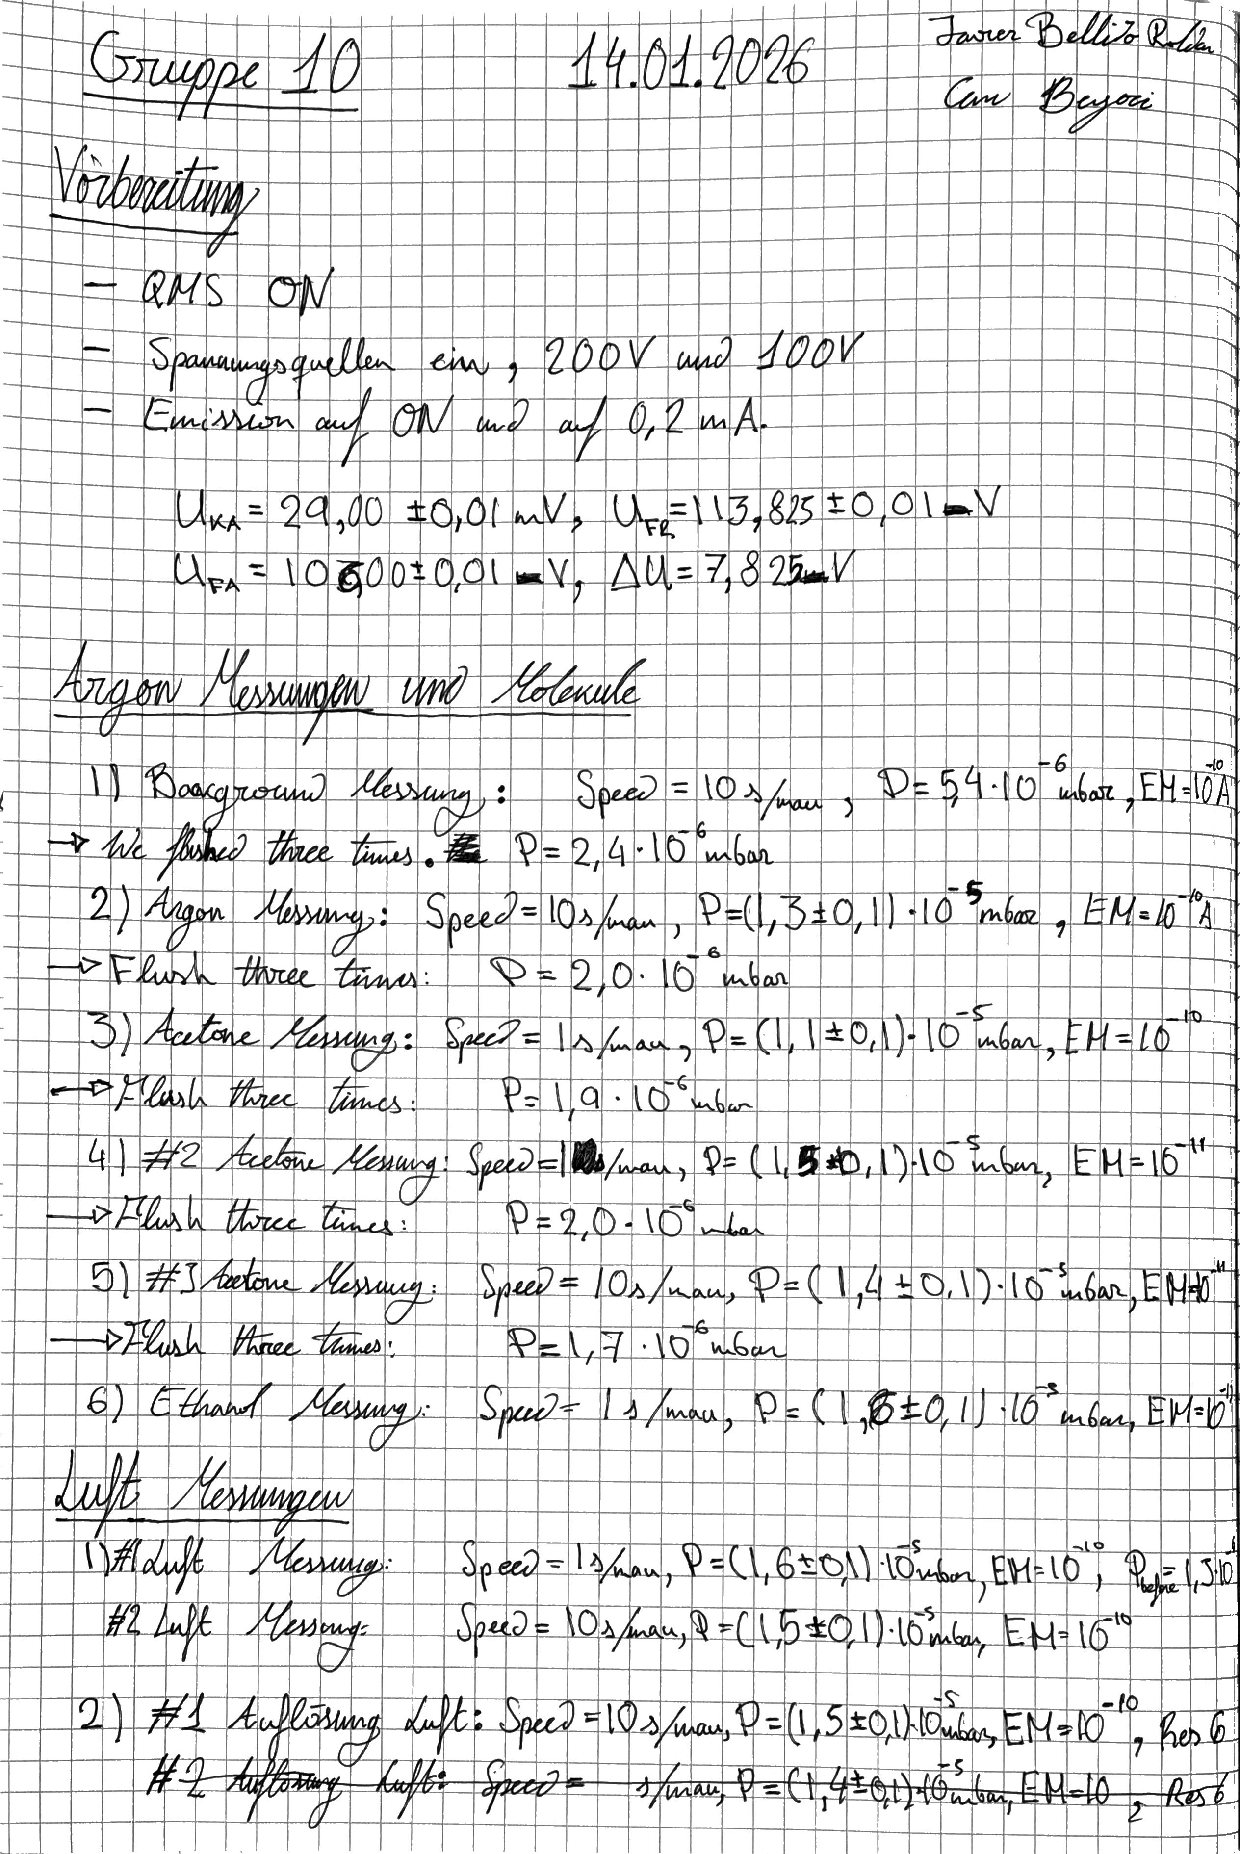
\includepdf[pages=-, scale=0.9, pagecommand={\thispagestyle{empty}}]{../resources/QMS_LabReport.pdf}

\end{document}
